\documentclass[journal]{IEEEtran}
\usepackage[a5paper, margin=10mm]{geometry}
%\usepackage{lmodern} % Ensure lmodern is loaded for pdflatex

\setlength{\headheight}{1cm} % Set the height of the header box
\setlength{\headsep}{0mm}     % Set the distance between the header box and the top of the text

%
\usepackage{gvv-book}
\usepackage{gvv}
\usetikzlibrary{patterns}
\lstset{aboveskip=12pt}
\usepackage[center]{caption}
\raggedbottom
\hypersetup{
    colorlinks=true,
    urlcolor=black % Changes text color instead of placing a box around it
}
\usepackage{amsfonts}
\makeindex

\begin{document}
\bibliographystyle{IEEEtran}
\onecolumn


\title{
	%\begin{flushleft}
	\begin{center}
	%MATRICES \\ In Geometry
	Math for EE
	\\
\rule{0.4\columnwidth}{0.4pt}
%\end{flushleft}
\end{center}
}
\author{
\vspace{11cm}
	%\begin{flushleft}
	\begin{center}
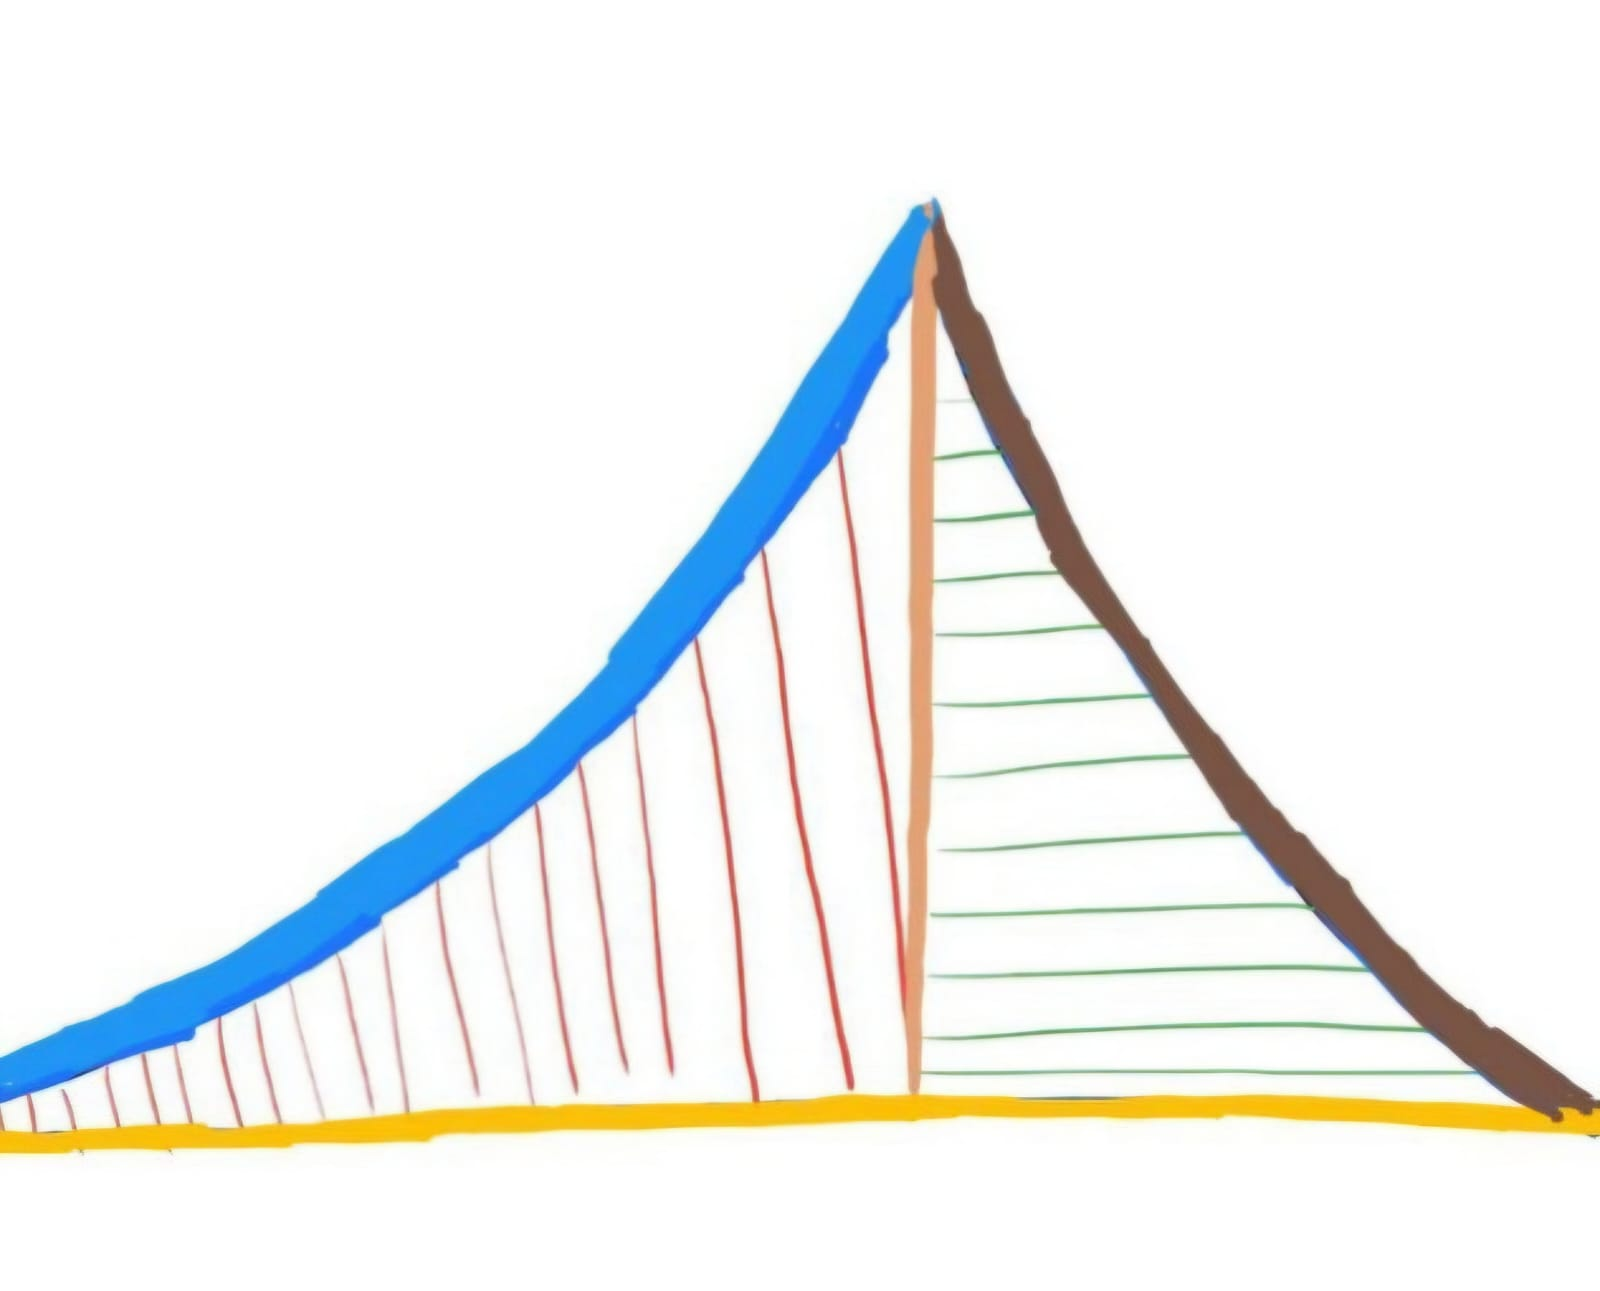
\includegraphics[width=0.2\columnwidth]{figs/logo.jpg}
\\
		{	\huge G. V. V. Sharma}
	\end{center}
	%\end{flushleft}
}
\maketitle

\newpage
\section*{About this Book}

This book contains solutions to the questions of the CBSE Class 10 Maths (Standard) paper 30/C/3 and the CBSE Class 12 Mathematics paper 65/C/3. Each solution is written with vectors and is verified numerically with Python or C codes. Roots are found by the Newton-Raphson method, linear equations are solved by Gauss elimination, definite integrals are evaluated by the trapezoidal rule, probability problems use the pmf and derivatives are checked with the Laplace transform and the Euler forward difference.

Each chapter has a formulae section and a problems section. The codes are in the folders \texttt{class10/codes} and \texttt{class12/codes} and the figures are in the folders \texttt{class10/figs} and \texttt{class12/figs}.

\newpage


\tableofcontents

\newpage
\onecolumn

\numberwithin{equation}{enumi}
\numberwithin{figure}{enumi}
\renewcommand{\thetable}{\theenumi}

% ---------------- Class 10 ----------------
% problems.tex refers to figures as figs/qN.png, so the graphics path is set to the class folder
\graphicspath{{class10/}}
\section{CBSE Class 10 Maths (Standard) 30/C/3}
\subsection{Formulae}
\begin{enumerate}[label=\thesubsection.\arabic*, ref=\thesubsection.\theenumi,itemsep=0pt]

\item The unit step sequence is defined as
\begin{align}
u(n) = \begin{cases} 1 & n \ge 0 \\ 0 & n < 0 \end{cases}
\label{eq:cb10-step}
\end{align}

\item An arithmetic progression (AP) with first term $a$ and common difference $d$ is the sequence
\begin{align}
x(n) = \brak{a + \brak{n-1}d}\, u(n-1)
\label{eq:cb10-ap-term}
\end{align}
The sum of the first $N$ terms is
\begin{align}
S_N = \sum_{n=-\infty}^{\infty} x(n)\sbrak{u(n-1) - u(n-N-1)} = \frac{N}{2}\brak{2a + \brak{N-1}d}
\label{eq:cb10-ap-sum}
\end{align}
\solution The window $u(n-1) - u(n-N-1)$ is $1$ only for $1 \le n \le N$. Hence
\begin{align}
S_N = \sum_{n=1}^{N}\brak{a + \brak{n-1}d} = Na + d\frac{N\brak{N-1}}{2}
\end{align}
yielding \eqref{eq:cb10-ap-sum}.

\item If $x(n-1), x(n), x(n+1)$ are consecutive terms of an AP, then
\begin{align}
x(n) = \frac{x(n-1) + x(n+1)}{2}
\label{eq:cb10-ap-mid}
\end{align}
\solution From \eqref{eq:cb10-ap-term}, $x(n+1) - x(n) = x(n) - x(n-1) = d$.

\item The direction vector of the line through $\vec{A}$ and $\vec{B}$, its normal vector and the distance between the points are
\begin{align}
\vec{m} = \vec{B} - \vec{A}, \quad \vec{n} = \vec{\Omega}\vec{m}, \quad \vec{\Omega} = \myvec{0 & 1 \\ -1 & 0}, \quad \norm{\vec{B}-\vec{A}} = \sqrt{\brak{\vec{B}-\vec{A}}^{\top}\brak{\vec{B}-\vec{A}}}
\label{eq:cb10-dir-norm}
\end{align}
with $\vec{m}^{\top}\vec{n} = 0$. The line in normal form is $\vec{n}^{\top}\vec{x} = c$ and in parametric form $\vec{x} = \vec{A} + \kappa\vec{m}$.

\item The mid point of $\vec{A}, \vec{B}$ is $\vec{C} = \dfrac{\vec{A}+\vec{B}}{2}$. Given $\vec{A}$ and the mid point $\vec{C}$, the other end point is
\begin{align}
\vec{B} = 2\vec{C} - \vec{A}
\label{eq:cb10-mid}
\end{align}
The point dividing $\vec{A}, \vec{B}$ in the ratio $k:1$ is $\dfrac{k\vec{B}+\vec{A}}{k+1}$.

\item The points $\vec{A}, \vec{B}, \vec{C}$ are collinear if
\begin{align}
\vec{B} - \vec{A} = k\brak{\vec{C} - \vec{A}} \quad \Longleftrightarrow \quad \rank\myvec{\vec{B}-\vec{A} & \vec{C}-\vec{A}} = 1
\label{eq:cb10-collinear}
\end{align}

\item The area of the triangle with vertices $\vec{A}, \vec{B}, \vec{C}$ is
\begin{align}
\text{ar}\brak{ABC} = \frac{1}{2}\abs{\vec{n}^{\top}\brak{\vec{C}-\vec{A}}}, \quad \vec{n} = \vec{\Omega}\brak{\vec{B}-\vec{A}}
\label{eq:cb10-area}
\end{align}
\solution $\vec{n}^{\top}\brak{\vec{C}-\vec{A}}$ is $\norm{\vec{B}-\vec{A}}$ times the signed distance of $\vec{C}$ from the line $AB$. The area is half of base times height. The area of a quadrilateral is the sum of the areas of the triangles obtained from a diagonal.

\item The roots of $ax^2 + bx + c = 0$ are
\begin{align}
x = \frac{-b \pm \sqrt{D}}{2a}, \quad D = b^2 - 4ac
\label{eq:cb10-quad}
\end{align}
The roots are equal if and only if $D = 0$. If $\alpha, \beta$ are the roots,
\begin{align}
\alpha + \beta = -\frac{b}{a}, \quad \alpha\beta = \frac{c}{a}, \quad \frac{1}{\alpha} + \frac{1}{\beta} = \frac{\alpha+\beta}{\alpha\beta} = -\frac{b}{c}
\label{eq:cb10-quad-sum}
\end{align}

\item \textbf{Newton-Raphson method.} A root of $f(x) = 0$ is obtained from the iteration
\begin{align}
x_{n+1} = x_n - \frac{f\brak{x_n}}{f'\brak{x_n}}
\label{eq:cb10-nr}
\end{align}
starting from an initial guess $x_0$, until $\abs{x_{n+1}-x_n}$ is smaller than the tolerance.

\item \textbf{Gauss elimination.} The system $\vec{A}\vec{x} = \vec{b}$ is written as the augmented matrix and reduced by row operations to the upper triangular form
\begin{align}
\myvec{\vec{A} & \vec{b}} \xrightarrow{\text{row operations}} \myvec{\vec{U} & \vec{c}}
\label{eq:cb10-gauss}
\end{align}
For $2 \times 2$ systems the operation is $R_2 \leftarrow R_2 - \frac{a_{21}}{a_{11}}R_1$. The unknowns are then found by back substitution. No determinant is used.

\item The probability mass function (pmf) of a discrete random variable $X$ is $p_X(x) = \pr{X = x}$. Then
\begin{align}
\sum_{x} p_X(x) = 1, \quad \pr{X \in E} = \sum_{x \in E} p_X(x), \quad \pr{E'} = 1 - \pr{E}
\label{eq:cb10-pmf}
\end{align}
The probability of an impossible event is $0$ and that of a sure event is $1$.

\item If $X, Y$ are independent, the pmf of $S = X + Y$ is the convolution
\begin{align}
p_S(s) = \sum_{x} p_X(x)\, p_Y(s - x)
\label{eq:cb10-conv}
\end{align}
For a fair die, $p_X(x) = \dfrac{1}{6}$ for $x = 1, \dots, 6$.

\item The rotation matrix is
\begin{align}
\vec{R}(\theta) = \myvec{\cos\theta & -\sin\theta \\ \sin\theta & \cos\theta}
\label{eq:cb10-rot}
\end{align}

\item \textbf{Tangent to a circle.} Let $T$ be the point of contact of a tangent from $\vec{P}$ to the circle with centre $\vec{O}$ and radius $r$. Then the tangent is perpendicular to the radius and the length of the tangent is
\begin{align}
\brak{\vec{T}-\vec{O}}^{\top}\brak{\vec{P}-\vec{T}} = 0, \quad \norm{\vec{P}-\vec{T}}^2 = \norm{\vec{P}-\vec{O}}^2 - r^2
\label{eq:cb10-tangent}
\end{align}
\solution $\norm{\vec{P}-\vec{O}}^2 = \norm{\brak{\vec{P}-\vec{T}} + \brak{\vec{T}-\vec{O}}}^2 = \norm{\vec{P}-\vec{T}}^2 + r^2$ since the cross term vanishes.

\item The two points of contact of the tangents from $\vec{P}$ are obtained by rotating the unit vector along $\vec{OP}$ through $\pm\varphi$:
\begin{align}
\vec{T}_{\pm} = \vec{O} + r\,\vec{R}\brak{\pm\varphi}\frac{\vec{P}-\vec{O}}{\norm{\vec{P}-\vec{O}}}, \quad \cos\varphi = \frac{r}{\norm{\vec{P}-\vec{O}}}
\label{eq:cb10-tpoints}
\end{align}
\solution In the right triangle $OTP$, $\cos\angle TOP = \dfrac{r}{\norm{OP}}$. $\varphi$ is obtained by the Newton-Raphson method from \eqref{eq:cb10-nr} with $f(\varphi) = \cos\varphi - \dfrac{r}{\norm{OP}}$. The quadrilateral $OAPB$ has two right angles at $A$ and $B$, so
\begin{align}
\angle AOB + \angle APB = 180^\circ
\label{eq:cb10-quadsum}
\end{align}
The angle between two vectors is $\cos\theta = \dfrac{\vec{u}^{\top}\vec{v}}{\norm{\vec{u}}\norm{\vec{v}}}$.

\item \textbf{Similar triangles.} If $\triangle ABC \sim \triangle PQR$ then
\begin{align}
\frac{AB}{PQ} = \frac{BC}{QR} = \frac{CA}{RP} = k, \quad \frac{\text{ar}\brak{ABC}}{\text{ar}\brak{PQR}} = k^2
\label{eq:cb10-similar}
\end{align}
(SSS criterion: proportional sides imply equal angles.) If $PQ \parallel BC$ with $P, Q$ on $AB, AC$ (basic proportionality theorem),
\begin{align}
\frac{AP}{AB} = \frac{AQ}{AC} = \frac{PQ}{BC}
\label{eq:cb10-bpt}
\end{align}

\item For a right angle at $A$, $\norm{\vec{B}-\vec{C}}^2 = \norm{\vec{A}-\vec{B}}^2 + \norm{\vec{A}-\vec{C}}^2$ since $\brak{\vec{B}-\vec{A}}^{\top}\brak{\vec{C}-\vec{A}} = 0$.
\label{eq:cb10-pyth}

\item For a moderately skewed distribution, the empirical relation is
\begin{align}
\text{mode} = 3\,\text{median} - 2\,\text{mean} = \myvec{3 & -2}\myvec{\text{median} \\ \text{mean}}
\label{eq:cb10-mode}
\end{align}

\item For grouped data with $N$ observations, class width $h$, the median class is the class whose cumulative frequency first exceeds $N/2$:
\begin{align}
\text{median} = l + \frac{\frac{N}{2} - cf}{f}\,h
\label{eq:cb10-median}
\end{align}
where $l$ is the lower limit of the median class, $cf$ the cumulative frequency before it and $f$ its frequency. The `less than' ogive is the polyline through the points (upper class limit, cumulative frequency). The abscissa of its point with ordinate $N/2$ is the median.

\item \textbf{Polynomials.} For polynomials $f, g$ there are unique $q, r$ with
\begin{align}
f(x) = g(x)q(x) + r(x), \quad \deg r < \deg g
\label{eq:cb10-polydiv}
\end{align}
$f$ is divisible by $g$ iff $r = 0$, in which case the zeros of $f$ are the zeros of $g$ together with the zeros of $q$.

\item If $p = a^{e_1}b^{e_2}$, $q = a^{f_1}b^{f_2}$ ($a, b$ prime), writing the exponents as vectors,
\begin{align}
\text{LCM}\brak{p,q} \leftrightarrow \max\brak{\vec{e},\vec{f}}, \quad \text{HCF}\brak{p,q} \leftrightarrow \min\brak{\vec{e},\vec{f}}
\label{eq:cb10-lcm}
\end{align}
(element-wise maximum and minimum).

\item \textbf{Trapezoidal rule.} For $N$ sub-intervals of width $h = \dfrac{b-a}{N}$,
\begin{align}
\int_a^b f(x)\,dx \approx \frac{h}{2}\sbrak{f(x_0) + 2\sum_{i=1}^{N-1}f(x_i) + f(x_N)}
\label{eq:cb10-trap}
\end{align}
The area of a circle of radius $r$ is $\pi r^2$ and the volume of a solid of constant cross section $A$ and thickness $t$ is
\begin{align}
V = \int_0^t A\,dz
\label{eq:cb10-vol}
\end{align}
which is $At$ for a coin.

\item \textbf{Angle of depression.} A line of sight from $\vec{C}$ at an angle of depression $\theta$ has direction vector $\vec{d}\brak{\theta} = \myvec{\cos\theta \\ -\sin\theta}$, so the line is $\vec{x} = \vec{C} + \lambda\vec{d}\brak{\theta}$. A line meets the ground ($\vec{e}_2^{\top}\vec{x} = 0$) or a vertical line ($\vec{e}_1^{\top}\vec{x} = c$) by solving the $2\times 2$ system, by Gauss elimination \eqref{eq:cb10-gauss}.
\label{eq:cb10-depr}

\item \textbf{Work.} If $A$ and $B$ take $x$ and $y$ days alone, then together they take $T$ days where
\begin{align}
\frac{1}{x} + \frac{1}{y} = \frac{1}{T}
\label{eq:cb10-work}
\end{align}

\end{enumerate}

\newpage
\subsection{Problems}
\begin{enumerate}[label=\thesubsection.\arabic*, ref=\thesubsection.\theenumi,itemsep=0pt]

\item If $-\dfrac{5}{7}, a, 2$ are consecutive terms in an Arithmetic Progression, then the value of $a$ is
\hfill (CBSE X 30/C/3, Q2)
\begin{enumerate}[itemsep=0pt]
\begin{multicols}{4}
\item $\frac{9}{7}$
\item $\frac{9}{14}$
\item $\frac{19}{7}$
\item $\frac{19}{14}$
\end{multicols}
\end{enumerate}

\solution From \eqref{eq:cb10-ap-term}, with $x(0) = -\frac{5}{7}$, $x(1) = a$, $x(2) = 2$ and the sequence written as $x(n) = \brak{x_0 + nd}u(n)$,
\begin{align}
x_0 &= -\frac{5}{7}, \quad x_0 + 2d = 2 \\
\implies \myvec{1 & 0 \\ 1 & 2}\myvec{x_0 \\ d} &= \myvec{-\frac{5}{7} \\ 2}
\end{align}
Gauss elimination, $R_2 \leftarrow R_2 - R_1$,
\begin{align}
\myvec{1 & 0 & -\frac{5}{7} \\ 1 & 2 & 2} \xrightarrow{R_2 \leftarrow R_2 - R_1} \myvec{1 & 0 & -\frac{5}{7} \\ 0 & 2 & \frac{19}{7}}
\implies x_0 = -\frac{5}{7}, \quad d = \frac{19}{14}
\end{align}
Therefore
\begin{align}
a = x(1) = x_0 + d = -\frac{5}{7} + \frac{19}{14} = \frac{9}{14}
\end{align}
which agrees with \eqref{eq:cb10-ap-mid}: $a = \frac{1}{2}\brak{-\frac{5}{7}+2} = \frac{9}{14}$. Hence option (B). The following code verifies this.
\begin{lstlisting}[frame=single, basicstyle=\rmfamily, escapeinside={(*@}{@*)}]
(*@\makebox[\dimexpr\linewidth-2\fboxsep-2\fboxrule\relax][c]{codes/q2.py}@*)
\end{lstlisting}

\item In the figure, if tangents $PA$ and $PB$ from an external point $P$ to a circle with centre $O$ are inclined to each other at an angle of $80^\circ$, then $\angle AOB$ is equal to
\hfill (CBSE X 30/C/3, Q5)
\begin{enumerate}[itemsep=0pt]
\begin{multicols}{4}
\item $100^\circ$
\item $60^\circ$
\item $80^\circ$
\item $50^\circ$
\end{multicols}
\end{enumerate}

\solution Let the radius be $r$ (assumed $1$) and $\vec{O} = \vec{0}$, $\vec{P} = d\vec{e}_1$. In the right triangle $OAP$, $\angle APO = 40^\circ$,
\begin{align}
d = \frac{r}{\sin 40^\circ}, \quad \varphi = \angle AOP,\ \cos\varphi = \frac{r}{d} = \sin 40^\circ
\end{align}
$\varphi$ is found from the Newton-Raphson iteration \eqref{eq:cb10-nr} with $f(\varphi) = \cos\varphi - \dfrac{r}{d}$, giving $\varphi = 50^\circ$. From \eqref{eq:cb10-tpoints}, the points of contact are $\vec{A} = r\vec{R}(\varphi)\vec{e}_1$ and $\vec{B} = r\vec{R}(-\varphi)\vec{e}_1$. Then
\begin{align}
\cos\angle AOB = \frac{\brak{\vec{A}-\vec{O}}^{\top}\brak{\vec{B}-\vec{O}}}{r^2} = \cos 2\varphi
\implies \angle AOB = 100^\circ
\end{align}
This agrees with \eqref{eq:cb10-quadsum}, $\angle AOB = 180^\circ - 80^\circ = 100^\circ$. Hence option (A). The following code verifies this in \figref{fig:cb10-q5}.
\begin{lstlisting}[frame=single, basicstyle=\rmfamily, escapeinside={(*@}{@*)}]
(*@\makebox[\dimexpr\linewidth-2\fboxsep-2\fboxrule\relax][c]{codes/q5.py}@*)
\end{lstlisting}
\begin{figure}[H]
\centering
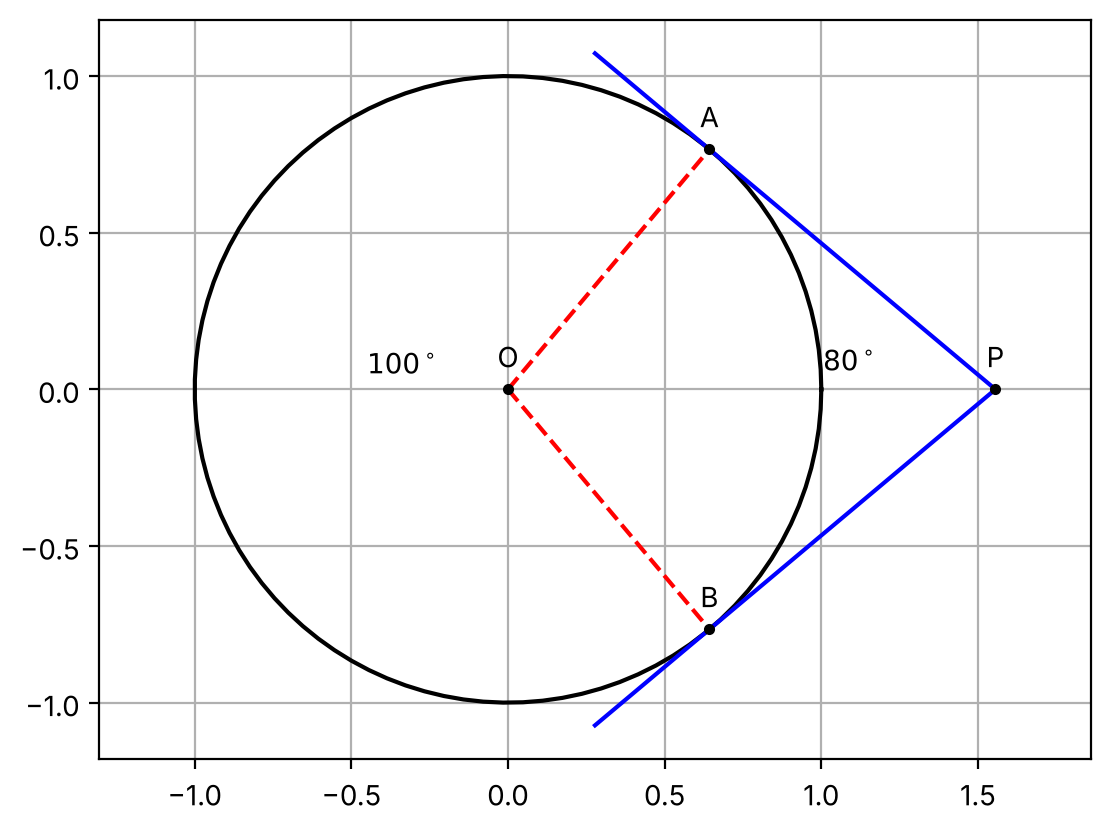
\includegraphics[width=0.60\linewidth]{figs/q5.png}
\caption{Tangents $PA$, $PB$ with $\angle APB = 80^\circ$}
\label{fig:cb10-q5}
\end{figure}

\item The mean and median of a distribution are $10$ and $14$ respectively. The value of the mode is
\hfill (CBSE X 30/C/3, Q6)
\begin{enumerate}[itemsep=0pt]
\begin{multicols}{4}
\item 6
\item 22
\item 2
\item 20
\end{multicols}
\end{enumerate}

\solution From \eqref{eq:cb10-mode},
\begin{align}
\text{mode} = \myvec{3 & -2}\myvec{14 \\ 10} = 42 - 20 = 22
\end{align}
Hence option (B). The following C code computes it as a dot product.
\begin{lstlisting}[frame=single, basicstyle=\rmfamily, escapeinside={(*@}{@*)}]
(*@\makebox[\dimexpr\linewidth-2\fboxsep-2\fboxrule\relax][c]{codes/q6.c}@*)
\end{lstlisting}

\item The value(s) of $k$ for which the quadratic equation $3x^2 - kx + 3 = 0$ has equal roots is (are)
\hfill (CBSE X 30/C/3, Q8)
\begin{enumerate}[itemsep=0pt]
\begin{multicols}{4}
\item 6
\item $-6$
\item $\pm 6$
\item 9
\end{multicols}
\end{enumerate}

\hfill OR \\
The discriminant of the quadratic equation $3\sqrt{3}x^2 + 10x + \sqrt{3} = 0$ is
\begin{enumerate}[itemsep=0pt]
\begin{multicols}{4}
\item $\pm 8$
\item 8
\item $100 - 4\sqrt{3}$
\item 64
\end{multicols}
\end{enumerate}

\solution From \eqref{eq:cb10-quad}, the roots are equal when
\begin{align}
D(k) = k^2 - 4\brak{3}\brak{3} = k^2 - 36 = 0
\end{align}
Applying the Newton-Raphson iteration \eqref{eq:cb10-nr} with $f(k) = k^2 - 36$, $f'(k) = 2k$,
\begin{align}
k_{n+1} = k_n - \frac{k_n^2 - 36}{2k_n} = \frac{1}{2}\brak{k_n + \frac{36}{k_n}}
\end{align}
Starting from $k_0 = 10$ the iteration converges to $k = 6$ and from $k_0 = -10$ to $k = -6$. Hence option (C), $k = \pm 6$.

\textbf{OR:} With $a = 3\sqrt{3}$, $b = 10$, $c = \sqrt{3}$,
\begin{align}
D = b^2 - 4ac = 100 - 4\brak{3\sqrt{3}}\brak{\sqrt{3}} = 100 - 36 = 64
\end{align}
Hence option (D). The following code verifies both parts in \figref{fig:cb10-q8}.
\begin{lstlisting}[frame=single, basicstyle=\rmfamily, escapeinside={(*@}{@*)}]
(*@\makebox[\dimexpr\linewidth-2\fboxsep-2\fboxrule\relax][c]{codes/q8.py}@*)
\end{lstlisting}
\begin{figure}[H]
\centering
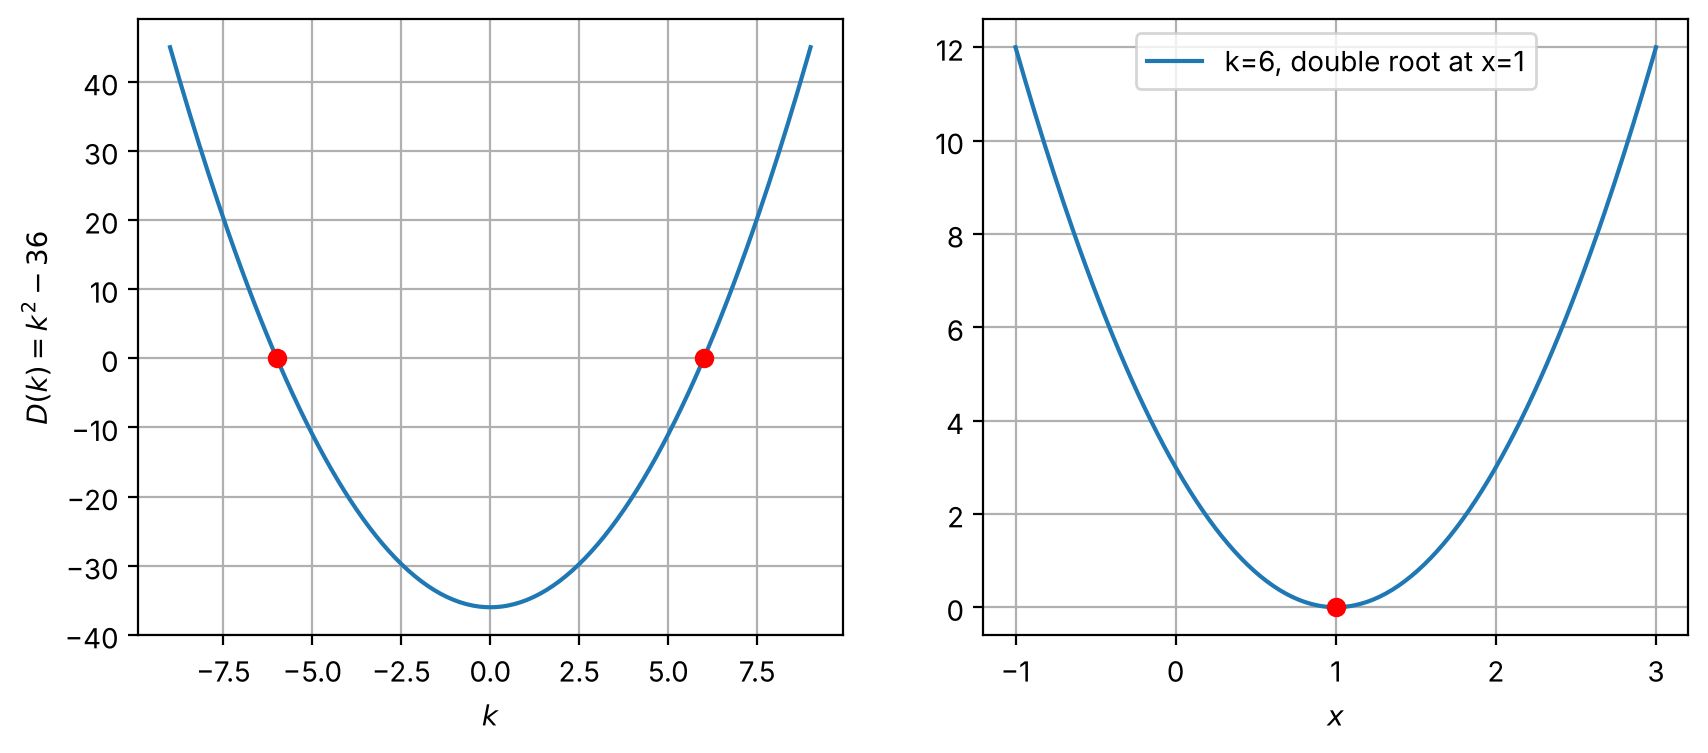
\includegraphics[width=0.80\linewidth]{figs/q8.png}
\caption{$D(k) = k^2 - 36$ and the double root of $3x^2 - 6x + 3$}
\label{fig:cb10-q8}
\end{figure}

\item Two dice are thrown simultaneously. The probability that the sum of the two numbers appearing on the top of the dice is less than $12$ is
\hfill (CBSE X 30/C/3, Q9)
\begin{enumerate}[itemsep=0pt]
\begin{multicols}{4}
\item $\frac{1}{36}$
\item $\frac{35}{36}$
\item 0
\item 1
\end{multicols}
\end{enumerate}

\solution Let $X, Y$ be the numbers on the two dice, each with $p_X(x) = p_Y(x) = \frac{1}{6}$. From \eqref{eq:cb10-conv}, the pmf of $S = X+Y$ is
\begin{align}
p_S(s) = \frac{\min\brak{s-1,\,13-s}}{36}, \quad s = 2, \dots, 12
\end{align}
and $p_S(12) = \frac{1}{36}$. From \eqref{eq:cb10-pmf},
\begin{align}
\pr{S < 12} = 1 - p_S(12) = 1 - \frac{1}{36} = \frac{35}{36}
\end{align}
Hence option (B). The following code computes the pmf by convolution in \figref{fig:cb10-q9}.
\begin{lstlisting}[frame=single, basicstyle=\rmfamily, escapeinside={(*@}{@*)}]
(*@\makebox[\dimexpr\linewidth-2\fboxsep-2\fboxrule\relax][c]{codes/q9.py}@*)
\end{lstlisting}
\begin{figure}[H]
\centering
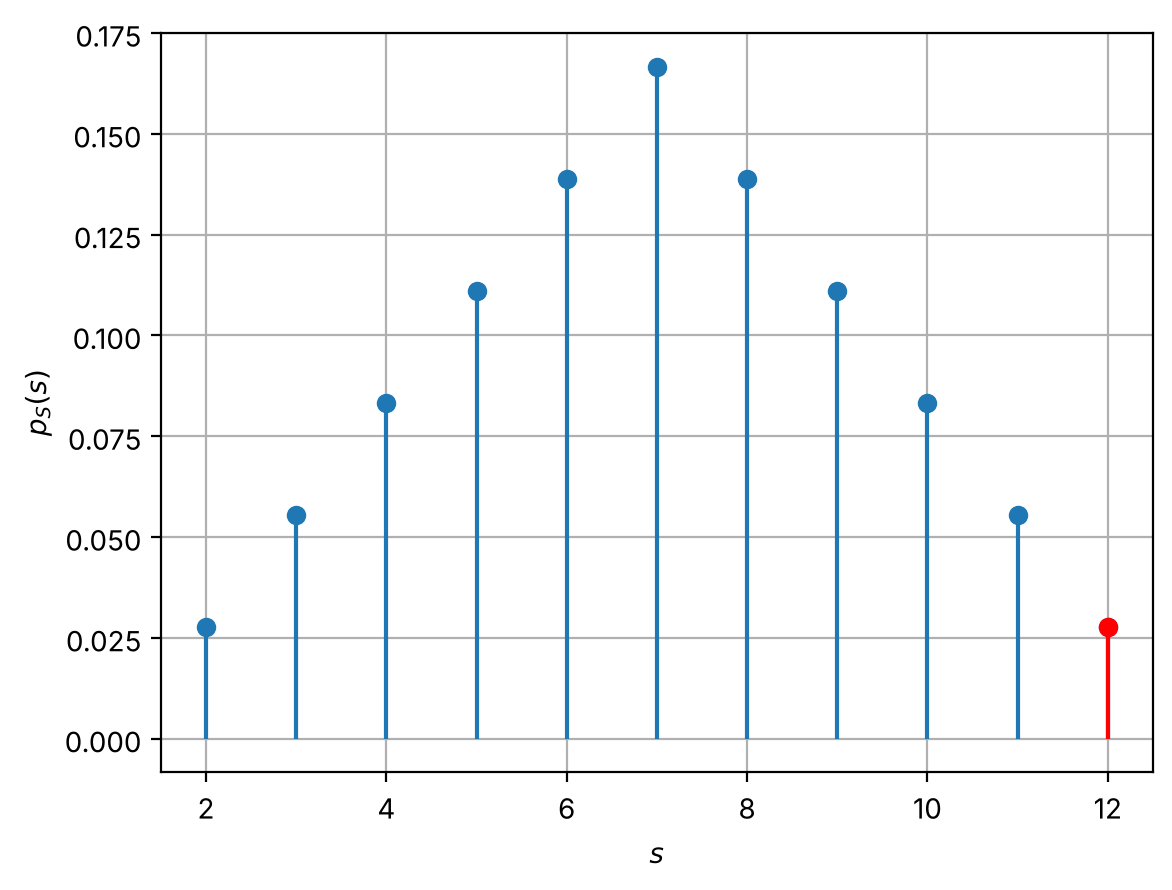
\includegraphics[width=0.60\linewidth]{figs/q9.png}
\caption{pmf of the sum of two dice}
\label{fig:cb10-q9}
\end{figure}

\item The value of $m$ which makes the points $\brak{0,0}$, $\brak{2m,-4}$ and $\brak{3,6}$ collinear is \underline{\hspace{1.5cm}}.
\hfill (CBSE X 30/C/3, Q14)

\solution Let $\vec{A} = \myvec{0 \\ 0}$, $\vec{B} = \myvec{2m \\ -4}$, $\vec{C} = \myvec{3 \\ 6}$. From \eqref{eq:cb10-collinear},
\begin{align}
\vec{B} - \vec{A} = k\brak{\vec{C} - \vec{A}}
\implies \myvec{2m \\ -4} = k\myvec{3 \\ 6}
\implies \myvec{2 & -3 \\ 0 & 6}\myvec{m \\ k} = \myvec{0 \\ -4}
\end{align}
This is already upper triangular, so by back substitution
\begin{align}
6k = -4 \implies k = -\frac{2}{3}, \quad 2m = 3k = -2 \implies m = -1
\end{align}
The points are $\brak{0,0}$, $\brak{-2,-4}$ and $\brak{3,6}$, which lie on one line. The following code verifies this in \figref{fig:cb10-q14}.
\begin{lstlisting}[frame=single, basicstyle=\rmfamily, escapeinside={(*@}{@*)}]
(*@\makebox[\dimexpr\linewidth-2\fboxsep-2\fboxrule\relax][c]{codes/q14.py}@*)
\end{lstlisting}
\begin{figure}[H]
\centering
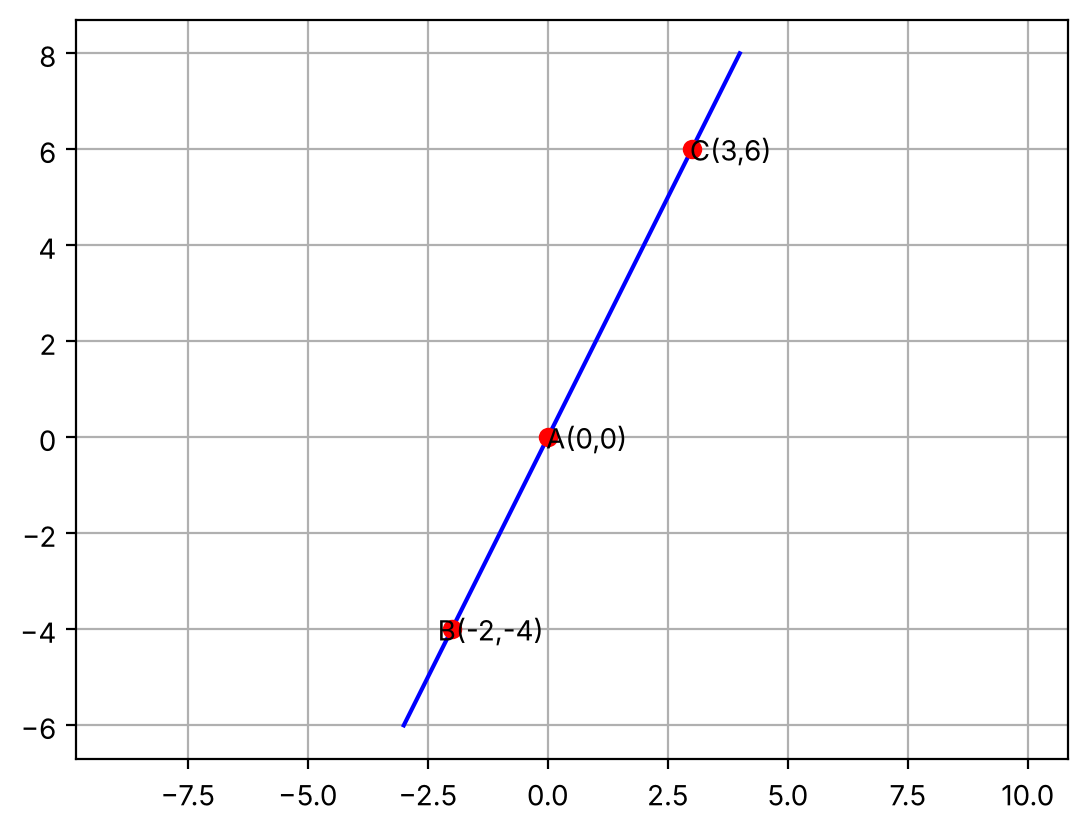
\includegraphics[width=0.55\linewidth]{figs/q14.png}
\caption{Collinear points for $m = -1$}
\label{fig:cb10-q14}
\end{figure}

\item If $\alpha, \beta$ are zeroes of the polynomial $2x^2 - 5x - 4$, then $\dfrac{1}{\alpha} + \dfrac{1}{\beta} = $ \underline{\hspace{1.5cm}}.
\hfill (CBSE X 30/C/3, Q15)

\solution From \eqref{eq:cb10-quad-sum} with $a = 2$, $b = -5$, $c = -4$,
\begin{align}
\alpha + \beta = \frac{5}{2}, \quad \alpha\beta = -2
\implies \frac{1}{\alpha} + \frac{1}{\beta} = \frac{\alpha+\beta}{\alpha\beta} = \frac{5/2}{-2} = -\frac{5}{4}
\end{align}
The roots are found numerically by the Newton-Raphson iteration \eqref{eq:cb10-nr},
\begin{align}
x_{n+1} = x_n - \frac{2x_n^2 - 5x_n - 4}{4x_n - 5}
\end{align}
giving $\alpha = 3.1375$ (from $x_0 = 3$) and $\beta = -0.6375$ (from $x_0 = -1$), so $\frac{1}{\alpha} + \frac{1}{\beta} = -1.25$. The following code verifies this in \figref{fig:cb10-q15}.
\begin{lstlisting}[frame=single, basicstyle=\rmfamily, escapeinside={(*@}{@*)}]
(*@\makebox[\dimexpr\linewidth-2\fboxsep-2\fboxrule\relax][c]{codes/q15.py}@*)
\end{lstlisting}
\begin{figure}[H]
\centering
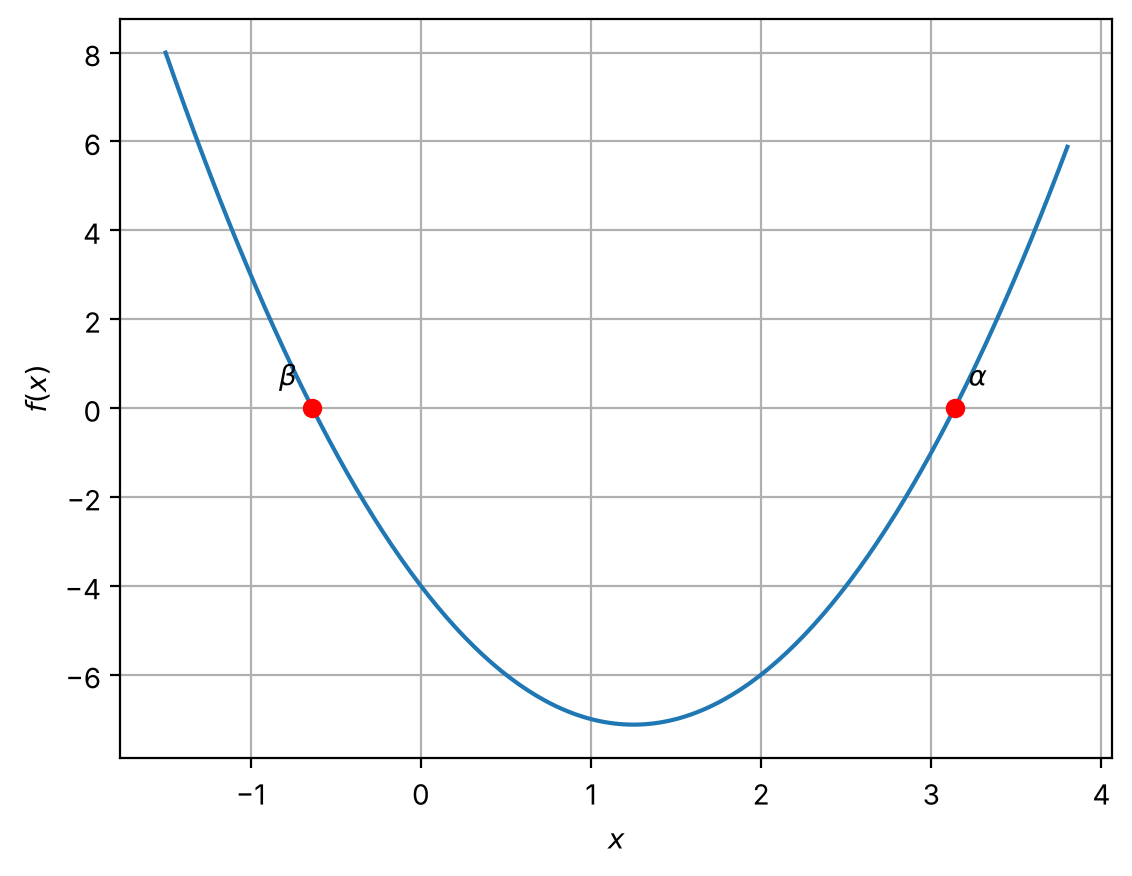
\includegraphics[width=0.55\linewidth]{figs/q15.png}
\caption{Zeroes of $2x^2 - 5x - 4$}
\label{fig:cb10-q15}
\end{figure}

\item A circle has its centre at $\brak{4,4}$. If one end of a diameter is $\brak{4,0}$, then find the coordinates of the other end.
\hfill (CBSE X 30/C/3, Q17)

\solution Let $\vec{C} = \myvec{4 \\ 4}$ and $\vec{A} = \myvec{4 \\ 0}$. The centre is the mid point of the diameter, so from \eqref{eq:cb10-mid},
\begin{align}
\vec{B} = 2\vec{C} - \vec{A} = \myvec{8 \\ 8} - \myvec{4 \\ 0} = \myvec{4 \\ 8}
\end{align}
The radius is $\norm{\vec{A}-\vec{C}} = 4 = \norm{\vec{B}-\vec{C}}$. The following code verifies this in \figref{fig:cb10-q17}.
\begin{lstlisting}[frame=single, basicstyle=\rmfamily, escapeinside={(*@}{@*)}]
(*@\makebox[\dimexpr\linewidth-2\fboxsep-2\fboxrule\relax][c]{codes/q17.py}@*)
\end{lstlisting}
\begin{figure}[H]
\centering
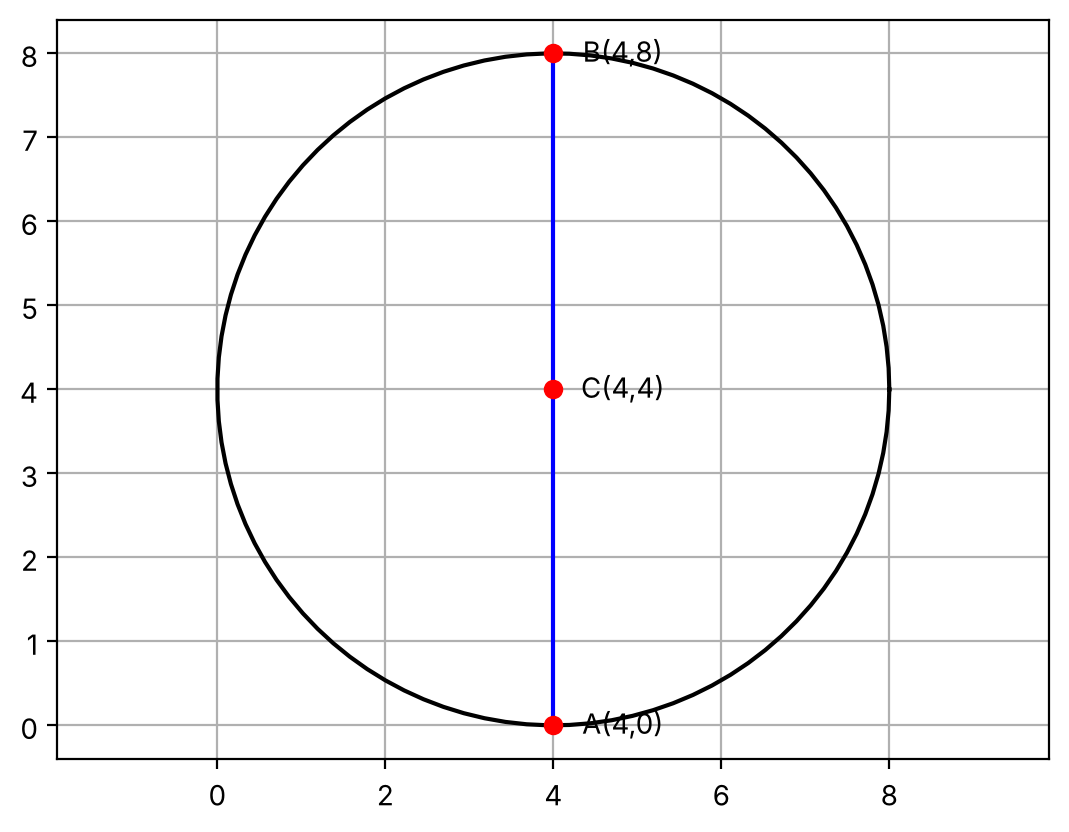
\includegraphics[width=0.45\linewidth]{figs/q17.png}
\caption{Circle with diameter $AB$}
\label{fig:cb10-q17}
\end{figure}

\item If two positive integers $p$ and $q$ can be expressed as $p = ab^3$ and $q = a^2b$, $a$ and $b$ being prime numbers, then find LCM$\brak{p,q}$.
\hfill (CBSE X 30/C/3, Q18)

\solution Writing the exponents of $\brak{a,b}$ as vectors, $\vec{e} = \myvec{1 \\ 3}$ for $p$ and $\vec{f} = \myvec{2 \\ 1}$ for $q$. From \eqref{eq:cb10-lcm},
\begin{align}
\max\brak{\vec{e},\vec{f}} = \myvec{\max\brak{1,2} \\ \max\brak{3,1}} = \myvec{2 \\ 3}
\implies \text{LCM}\brak{p,q} = a^2b^3
\end{align}
The following code verifies this for several prime pairs.
\begin{lstlisting}[frame=single, basicstyle=\rmfamily, escapeinside={(*@}{@*)}]
(*@\makebox[\dimexpr\linewidth-2\fboxsep-2\fboxrule\relax][c]{codes/q18.py}@*)
\end{lstlisting}

\item It is given that $\triangle ABC \sim \triangle PQR$ with $\dfrac{BC}{QR} = \dfrac{1}{3}$. Then find the value of $\dfrac{\text{ar}\brak{PRQ}}{\text{ar}\brak{ACB}}$.
\hfill (CBSE X 30/C/3, Q19)

\solution From \eqref{eq:cb10-similar} with $\dfrac{QR}{BC} = 3$,
\begin{align}
\frac{\text{ar}\brak{PRQ}}{\text{ar}\brak{ACB}} = \brak{\frac{QR}{BC}}^2 = 9
\end{align}
In the code, a triangle $\vec{A} = \myvec{1 \\ 1}, \vec{B} = \myvec{5 \\ 2}, \vec{C} = \myvec{3 \\ 6}$ is assumed and $\triangle PQR$ is obtained by the similarity $\vec{x} \to 3\vec{R}\brak{25^\circ}\vec{x} + \vec{t}$. The areas from \eqref{eq:cb10-area} are $9$ and $81$, whose ratio is $9$ in \figref{fig:cb10-q19}.
\begin{lstlisting}[frame=single, basicstyle=\rmfamily, escapeinside={(*@}{@*)}]
(*@\makebox[\dimexpr\linewidth-2\fboxsep-2\fboxrule\relax][c]{codes/q19.py}@*)
\end{lstlisting}
\begin{figure}[H]
\centering
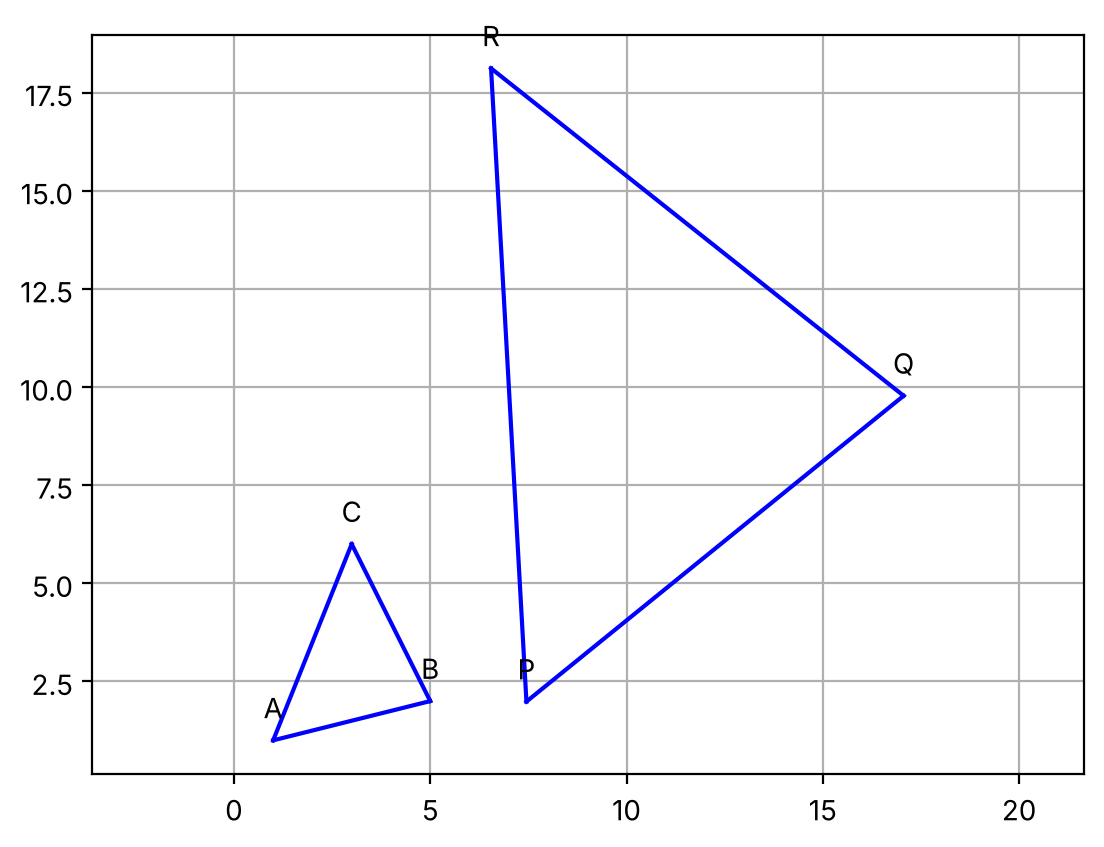
\includegraphics[width=0.55\linewidth]{figs/q19.png}
\caption{Similar triangles with ratio $1:3$}
\label{fig:cb10-q19}
\end{figure}

\item In the figure, $PQ \parallel BC$, $PQ = 3$ cm, $BC = 9$ cm and $AC = 7.5$ cm. Find the length of $AQ$.
\hfill (CBSE X 30/C/3, Q22)

\solution From \eqref{eq:cb10-bpt},
\begin{align}
\frac{AQ}{AC} = \frac{PQ}{BC} = \frac{3}{9} = \frac{1}{3}
\implies AQ = \frac{7.5}{3} = 2.5 \text{ cm}
\end{align}
In vector form, $\vec{Q} = \vec{A} + \frac{1}{3}\brak{\vec{C}-\vec{A}}$ and $\vec{P} = \vec{A} + \frac{1}{3}\brak{\vec{B}-\vec{A}}$, so $\vec{Q}-\vec{P} = \frac{1}{3}\brak{\vec{C}-\vec{B}}$, i.e. $PQ \parallel BC$ and $PQ = 3$. The triangle in \figref{fig:cb10-q22} is drawn with an assumed $AB = 6$ cm using the code below.
\begin{lstlisting}[frame=single, basicstyle=\rmfamily, escapeinside={(*@}{@*)}]
(*@\makebox[\dimexpr\linewidth-2\fboxsep-2\fboxrule\relax][c]{codes/q22.py}@*)
\end{lstlisting}
\begin{figure}[H]
\centering
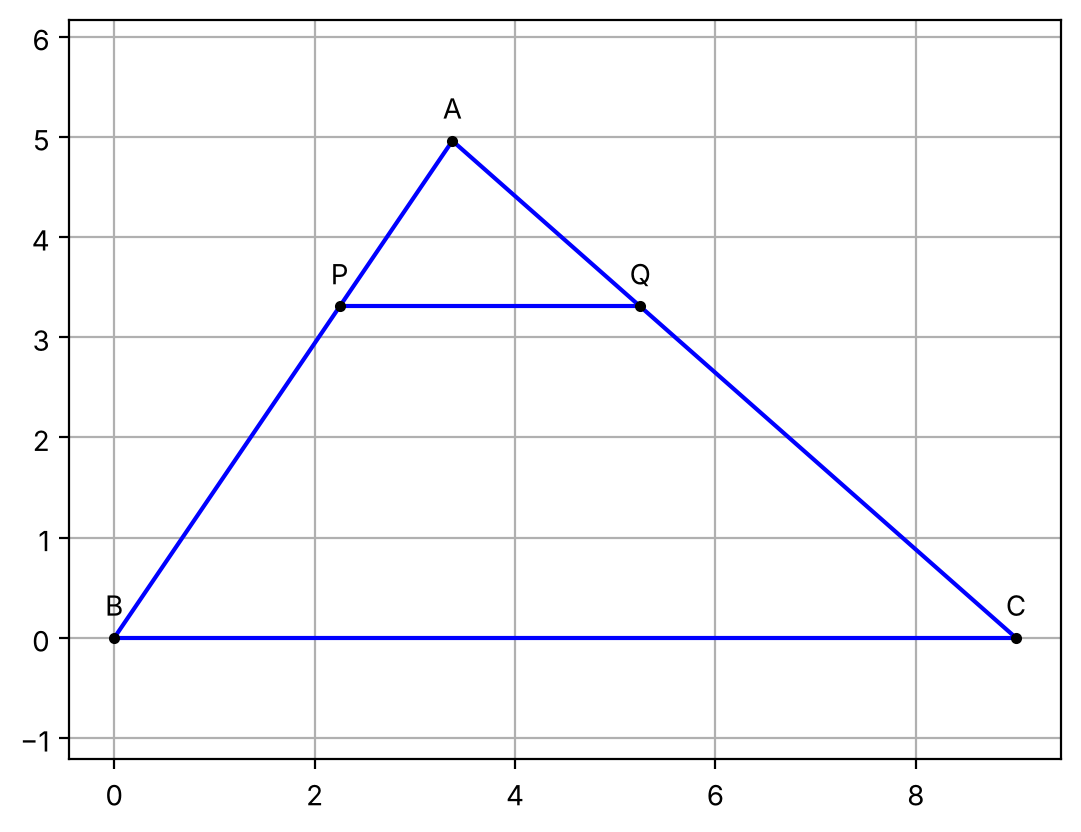
\includegraphics[width=0.60\linewidth]{figs/q22.png}
\caption{$PQ \parallel BC$}
\label{fig:cb10-q22}
\end{figure}

\item Solve $9x^2 - 6a^2x + a^4 - b^4 = 0$ using the quadratic formula.
\hfill (CBSE X 30/C/3, Q23)

\solution Here $A = 9$, $B = -6a^2$, $C = a^4 - b^4$. From \eqref{eq:cb10-quad},
\begin{align}
D &= 36a^4 - 36\brak{a^4 - b^4} = 36b^4 \\
x &= \frac{6a^2 \pm 6b^2}{18} = \frac{a^2 \pm b^2}{3}
\end{align}
Therefore the roots are $\dfrac{a^2+b^2}{3}$ and $\dfrac{a^2-b^2}{3}$. The code takes $a = 2$, $b = 1$ (roots $\frac{5}{3}, 1$), checks them with the Newton-Raphson iteration \eqref{eq:cb10-nr} and tests other values in \figref{fig:cb10-q23}.
\begin{lstlisting}[frame=single, basicstyle=\rmfamily, escapeinside={(*@}{@*)}]
(*@\makebox[\dimexpr\linewidth-2\fboxsep-2\fboxrule\relax][c]{codes/q23.py}@*)
\end{lstlisting}
\begin{figure}[H]
\centering
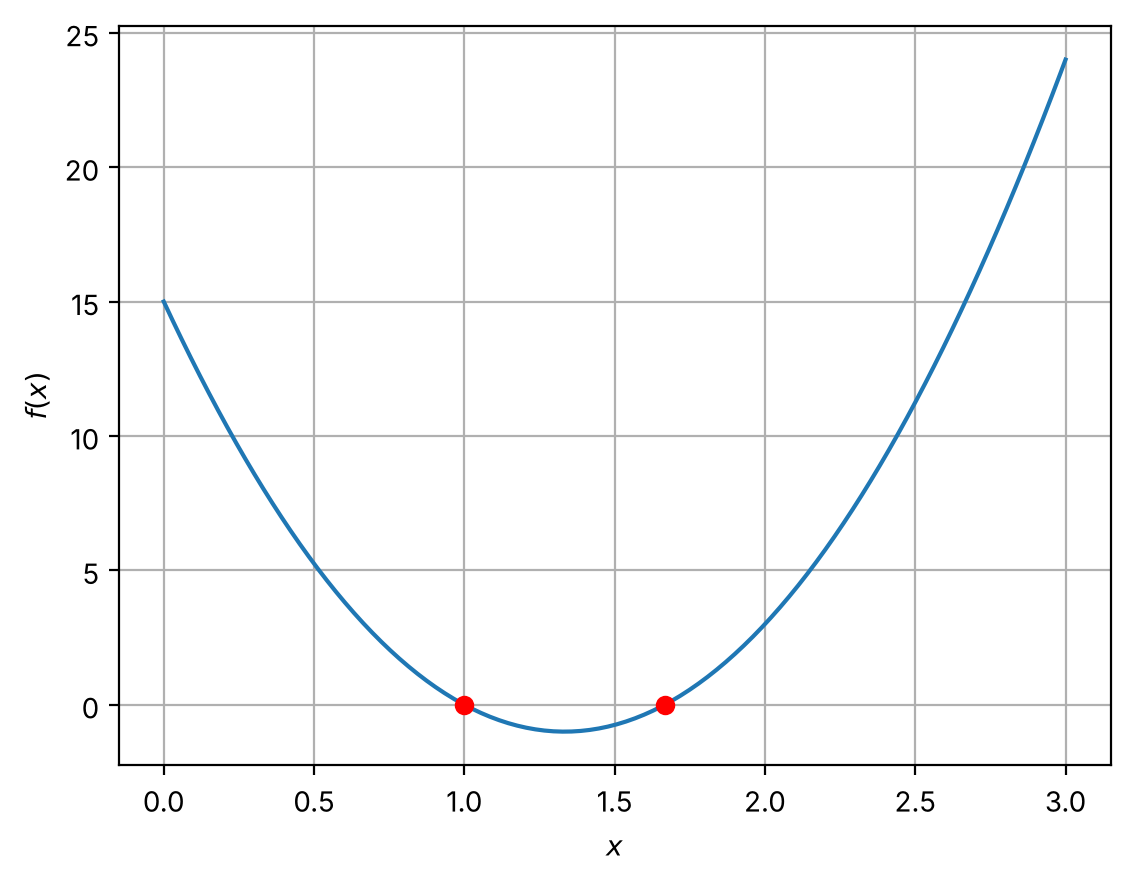
\includegraphics[width=0.50\linewidth]{figs/q23.png}
\caption{Roots of $9x^2 - 24x + 15 = 0$}
\label{fig:cb10-q23}
\end{figure}

\item A jar contains $18$ marbles. Some are red and others are yellow. If a marble is drawn at random from the jar, the probability that it is red is $\dfrac{2}{3}$. Find the number of yellow marbles in the jar.
\hfill (CBSE X 30/C/3, Q24)

\hfill OR \\
A die is thrown twice. What is the probability that (i) $5$ will come up at least once, and (ii) $5$ will not come up either time?

\solution Let $r$ and $y$ be the number of red and yellow marbles. The pmf of the marble drawn is $p(\text{red}) = \frac{r}{18}$, $p(\text{yellow}) = \frac{y}{18}$ with $p(\text{red}) = \frac{2}{3}$,
\begin{align}
r + y = 18, \quad r - 2y = 0
\implies \myvec{1 & 1 & 18 \\ 1 & -2 & 0} \xrightarrow{R_2 \leftarrow R_2 - R_1} \myvec{1 & 1 & 18 \\ 0 & -3 & -18}
\end{align}
Back substitution gives $y = 6$ and $r = 12$. There are $6$ yellow marbles.

\textbf{OR:} Let $X$ be the number of fives in a single throw, $p(1) = \frac{1}{6}$, $p(0) = \frac{5}{6}$. For two throws \eqref{eq:cb10-conv} gives the pmf of the number of fives
\begin{align}
p_2 = \myvec{\frac{5}{6} & \frac{1}{6}} * \myvec{\frac{5}{6} & \frac{1}{6}} = \myvec{\frac{25}{36} & \frac{10}{36} & \frac{1}{36}}
\end{align}
From \eqref{eq:cb10-pmf}, (ii) $\pr{\text{no } 5} = \frac{25}{36}$ and (i) $\pr{\text{at least one } 5} = 1 - \frac{25}{36} = \frac{11}{36}$. The following code verifies both in \figref{fig:cb10-q24}.
\begin{lstlisting}[frame=single, basicstyle=\rmfamily, escapeinside={(*@}{@*)}]
(*@\makebox[\dimexpr\linewidth-2\fboxsep-2\fboxrule\relax][c]{codes/q24.py}@*)
\end{lstlisting}
\begin{figure}[H]
\centering
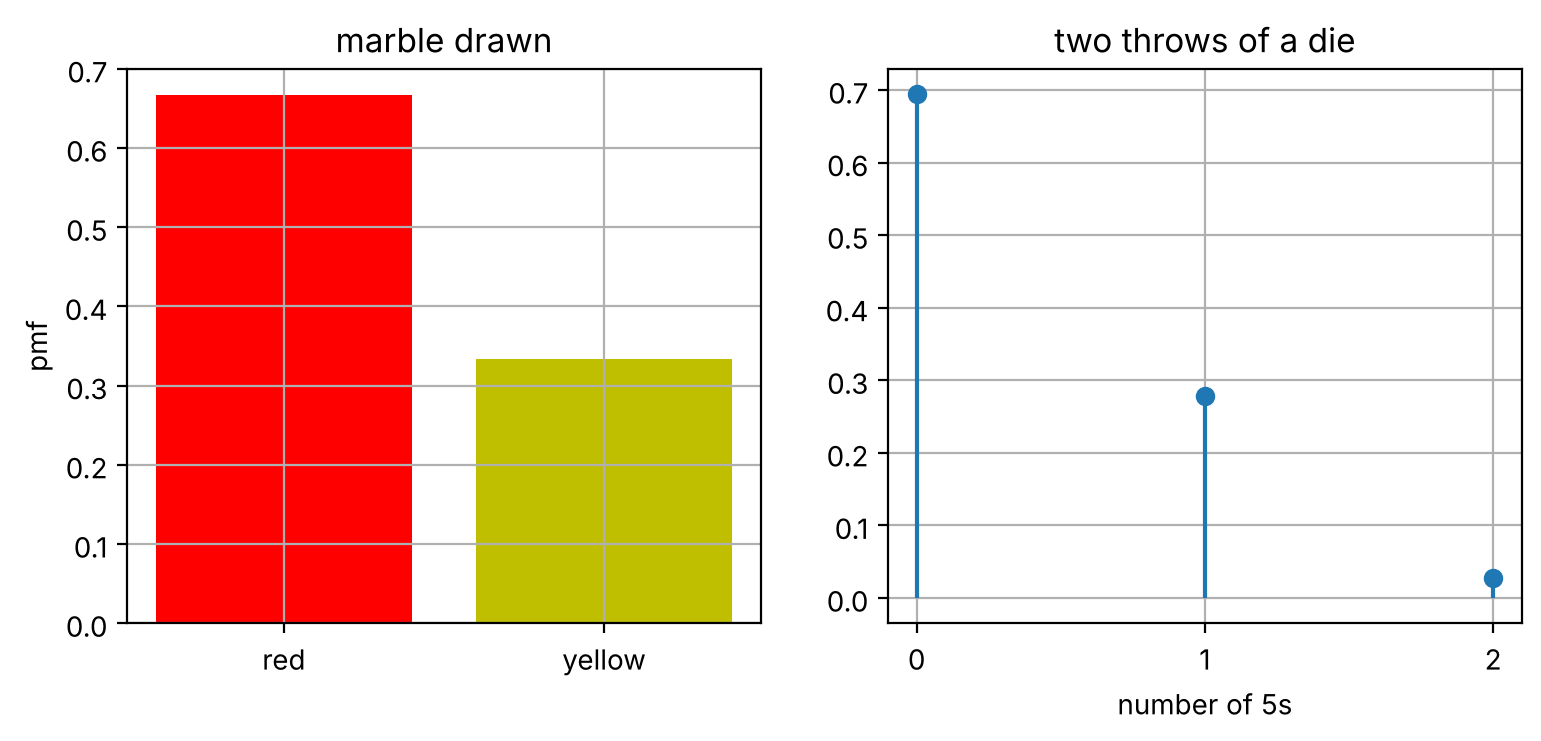
\includegraphics[width=0.75\linewidth]{figs/q24.png}
\caption{pmfs for the marbles and for two throws of a die}
\label{fig:cb10-q24}
\end{figure}

\item Find the area of the quadrilateral $ABCD$ whose vertices are $A\brak{-4,-3}$, $B\brak{3,-1}$, $C\brak{0,5}$ and $D\brak{-4,2}$.
\hfill (CBSE X 30/C/3, Q28)

\hfill OR \\
If the points $A\brak{2,0}$, $B\brak{6,1}$ and $C\brak{p,q}$ form a triangle of area $12$ sq. units (positive only) and $2p + q = 10$, then find the values of $p$ and $q$.

\solution The diagonal $AC$ divides $ABCD$ into $\triangle ABC$ and $\triangle ACD$. With $\vec{n} = \vec{\Omega}\brak{\vec{C}-\vec{A}} = \myvec{8 \\ -4}$, $\vec{n}^{\top}\brak{\vec{B}-\vec{A}} = 48$ and $\vec{n}^{\top}\brak{\vec{D}-\vec{A}} = -20$ have opposite signs, so $B$ and $D$ lie on opposite sides. From \eqref{eq:cb10-area},
\begin{align}
\text{ar}\brak{ABC} &= \frac{1}{2}\abs{\brak{\vec{\Omega}\brak{\vec{B}-\vec{A}}}^{\top}\brak{\vec{C}-\vec{A}}} = \frac{1}{2}\abs{\myvec{2 & -7}\myvec{4 \\ 8}} = 24 \\
\text{ar}\brak{ACD} &= \frac{1}{2}\abs{\myvec{8 & -4}\myvec{0 \\ 5}} = 10 \\
\text{ar}\brak{ABCD} &= 24 + 10 = 34 \text{ sq. units}
\end{align}

\textbf{OR:} $\vec{n} = \vec{\Omega}\brak{\vec{B}-\vec{A}} = \myvec{0 & 1 \\ -1 & 0}\myvec{4 \\ 1} = \myvec{1 \\ -4}$. From \eqref{eq:cb10-area},
\begin{align}
\frac{1}{2}\abs{\vec{n}^{\top}\brak{\vec{C}-\vec{A}}} = 12 \implies \vec{n}^{\top}\vec{C} = \vec{n}^{\top}\vec{A} \pm 24 = 2 \pm 24
\end{align}
Together with $2p + q = 10$, two linear systems result:
\begin{align}
\myvec{1 & -4 & 26 \\ 2 & 1 & 10} \xrightarrow{R_2 \leftarrow R_2 - 2R_1} \myvec{1 & -4 & 26 \\ 0 & 9 & -42}
\implies \myvec{p \\ q} = \myvec{\frac{22}{3} \\ -\frac{14}{3}} \\
\myvec{1 & -4 & -22 \\ 2 & 1 & 10} \xrightarrow{R_2 \leftarrow R_2 - 2R_1} \myvec{1 & -4 & -22 \\ 0 & 9 & 54}
\implies \myvec{p \\ q} = \myvec{2 \\ 6}
\end{align}
So $\brak{p,q} = \brak{2,6}$ or $\brak{\frac{22}{3}, -\frac{14}{3}}$. The following code verifies both parts in \figref{fig:cb10-q28}.
\begin{lstlisting}[frame=single, basicstyle=\rmfamily, escapeinside={(*@}{@*)}]
(*@\makebox[\dimexpr\linewidth-2\fboxsep-2\fboxrule\relax][c]{codes/q28.py}@*)
\end{lstlisting}
\begin{figure}[H]
\centering
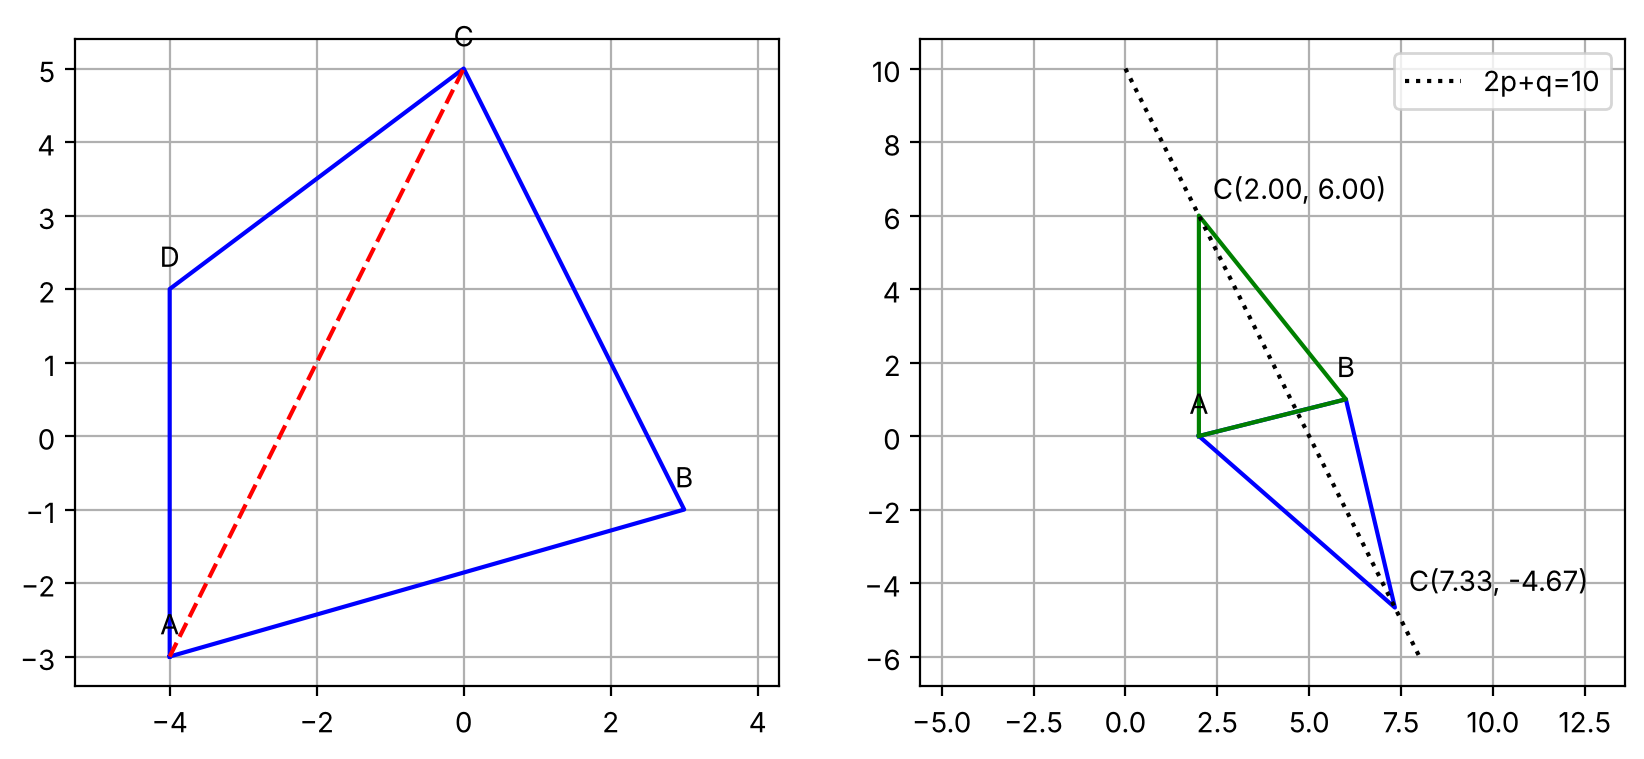
\includegraphics[width=0.85\linewidth]{figs/q28.png}
\caption{Quadrilateral $ABCD$ (left) and the two positions of $C$ (right)}
\label{fig:cb10-q28}
\end{figure}

\item Solve the equations $x + 2y = 6$ and $2x - 5y = 12$ graphically.
\hfill (CBSE X 30/C/3, Q30)

\hfill OR \\
Solve the following equations for $x$ and $y$ using the cross-multiplication method: $\brak{ax - by} + \brak{a + 4b} = 0$, $\brak{bx + ay} + \brak{b - 4a} = 0$.

\solution Each equation is a line $\vec{n}^{\top}\vec{x} = c$ with $\vec{n}_1 = \myvec{1 \\ 2}$, $c_1 = 6$ and $\vec{n}_2 = \myvec{2 \\ -5}$, $c_2 = 12$. The lines are plotted in \figref{fig:cb10-q30} using the parametric form $\vec{x} = \vec{h} + \kappa\vec{m}$ with $\vec{m} = \vec{\Omega}\vec{n}$ from \eqref{eq:cb10-dir-norm}. The point of intersection satisfies, by Gauss elimination \eqref{eq:cb10-gauss},
\begin{align}
\myvec{1 & 2 & 6 \\ 2 & -5 & 12} \xrightarrow{R_2 \leftarrow R_2 - 2R_1} \myvec{1 & 2 & 6 \\ 0 & -9 & 0}
\implies y = 0, \quad x = 6
\end{align}
The lines intersect at $\brak{6, 0}$.

\textbf{OR:} The equations are $ax - by = -\brak{a+4b}$ and $bx + ay = 4a - b$. Applying Gauss elimination with $R_2 \leftarrow R_2 - \frac{b}{a}R_1$ ($a \neq 0$),
\begin{align}
\myvec{a & -b & -\brak{a+4b} \\ b & a & 4a - b} \longrightarrow
\myvec{a & -b & -\brak{a+4b} \\ 0 & \frac{a^2+b^2}{a} & \frac{4\brak{a^2+b^2}}{a}}
\end{align}
Thus $y = 4$ and then $ax = -\brak{a + 4b} + 4b = -a$, so $x = -1$. The solution is $\brak{x,y} = \brak{-1,4}$ for every $a, b$ with $a^2 + b^2 \neq 0$. The following code solves both parts (the second one for assumed $a = 2$, $b = 3$ and other values) in \figref{fig:cb10-q30}.
\begin{lstlisting}[frame=single, basicstyle=\rmfamily, escapeinside={(*@}{@*)}]
(*@\makebox[\dimexpr\linewidth-2\fboxsep-2\fboxrule\relax][c]{codes/q30.py}@*)
\end{lstlisting}
\begin{figure}[H]
\centering
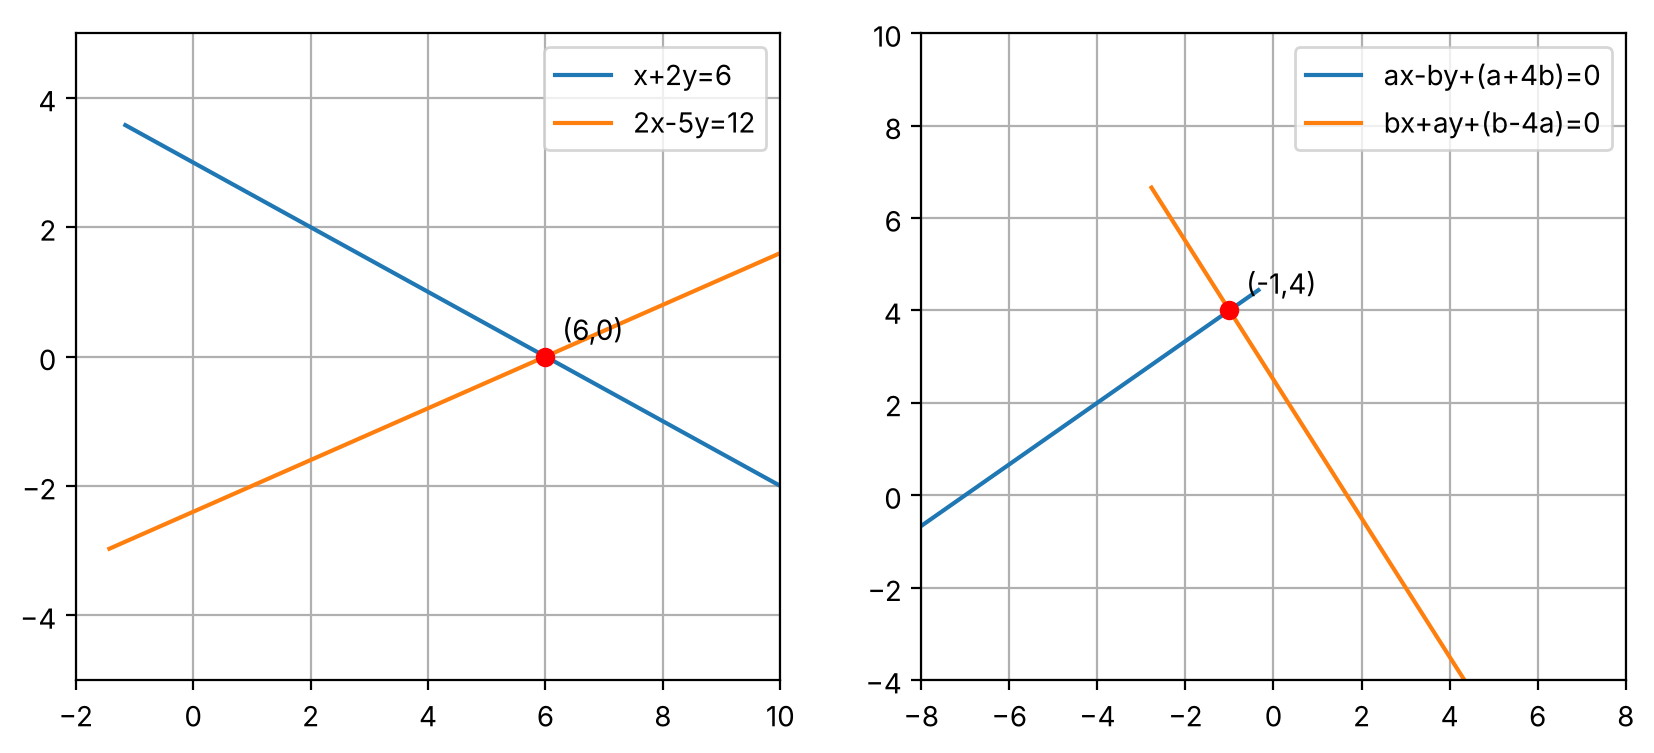
\includegraphics[width=0.85\linewidth]{figs/q30.png}
\caption{Graphical solutions $\brak{6,0}$ and $\brak{-1,4}$}
\label{fig:cb10-q30}
\end{figure}

\item Draw a circle of radius $2.5$ cm. Take a point $P$ outside the circle at a distance of $7$ cm from the centre. Then construct a pair of tangents to the circle from point $P$.
\hfill (CBSE X 30/C/3, Q31)

\solution Take $\vec{O} = \vec{0}$, $r = 2.5$ and $\vec{P} = 7\vec{e}_1$.

\textit{Construction:}
\begin{enumerate}[itemsep=0pt]
\item Draw the circle with centre $O$ and radius $2.5$ cm and mark $P$ with $OP = 7$ cm.
\item Find the mid point $\vec{M} = \frac{\vec{O}+\vec{P}}{2}$ of $OP$.
\item Draw the circle with centre $M$ and radius $MO = 3.5$ cm. It meets the first circle at $T_1, T_2$.
\item Join $PT_1$ and $PT_2$. These are the required tangents.
\end{enumerate}
\textit{Justification:} $T_1$ lies on the circle with diameter $OP$, so $\angle OT_1P = 90^\circ$, i.e. $\brak{\vec{T}_1 - \vec{O}}^{\top}\brak{\vec{P}-\vec{T}_1} = 0$ in \eqref{eq:cb10-tangent}. Numerically, from \eqref{eq:cb10-tpoints} $\cos\varphi = \frac{2.5}{7}$, which the Newton-Raphson iteration \eqref{eq:cb10-nr} solves as $\varphi = 69.075^\circ$ and
\begin{align}
\vec{T}_{1,2} = 2.5\,\vec{R}\brak{\pm\varphi}\vec{e}_1 = \myvec{0.893 \\ \pm 2.335}, \quad
\norm{\vec{P} - \vec{T}} = \sqrt{49 - 6.25} = 6.538 \text{ cm}
\end{align}
The following code draws the construction in \figref{fig:cb10-q31}.
\begin{lstlisting}[frame=single, basicstyle=\rmfamily, escapeinside={(*@}{@*)}]
(*@\makebox[\dimexpr\linewidth-2\fboxsep-2\fboxrule\relax][c]{codes/q31.py}@*)
\end{lstlisting}
\begin{figure}[H]
\centering
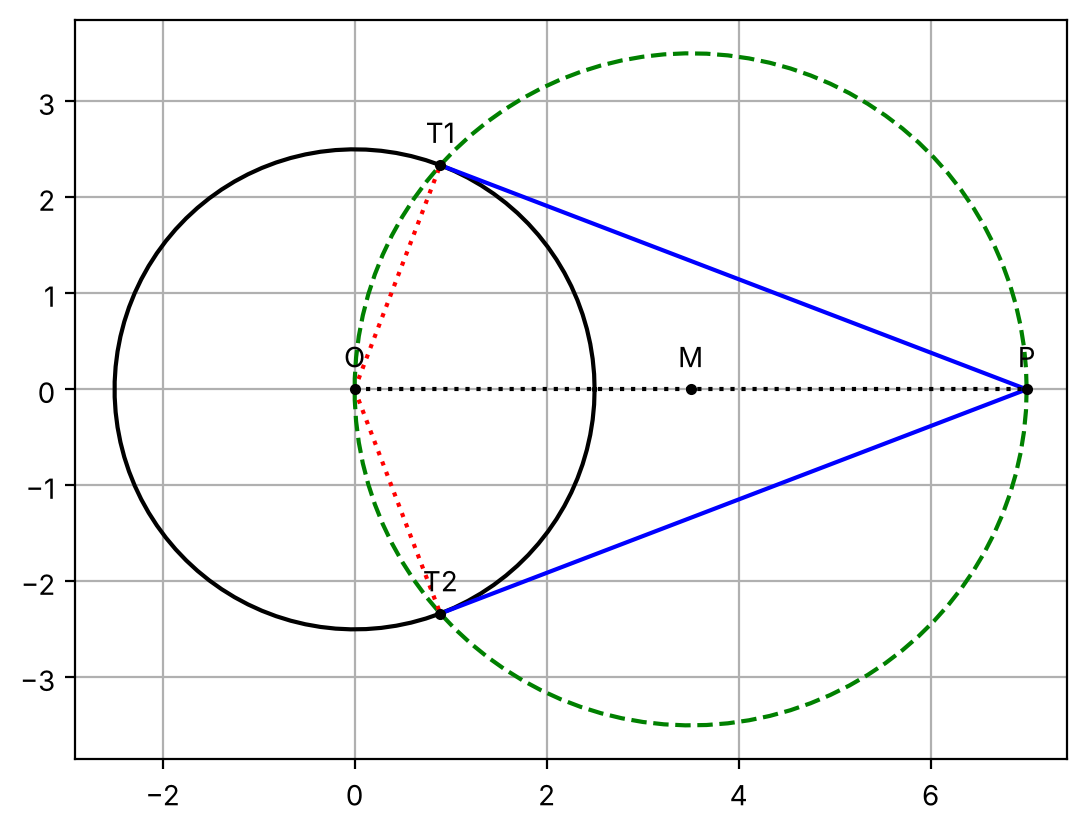
\includegraphics[width=0.80\linewidth]{figs/q31.png}
\caption{Tangents from $P$ to the circle}
\label{fig:cb10-q31}
\end{figure}

\item A mint moulds four types of copper coins $A, B, C$ and $D$ whose diameters vary from $0.5$ cm to $5$ cm. The first coin $A$ has a diameter of $0.7$ cm. The second coin $B$ has double the diameter of coin $A$ and from then onwards the diameters increase by $50\%$. Thickness of each coin is $0.25$ cm. (i) Fill in the diameter of coin $B$. (ii) Complete the table of the area (in cm$^2$) of one face and the volume (in cm$^3$) of coin $B$. [Use $\pi = \frac{22}{7}$]
\hfill (CBSE X 30/C/3, Q32)

\solution The diameters form the vector
\begin{align}
\vec{d} = \myvec{d_A \\ d_B \\ d_C \\ d_D} = \myvec{0.7 \\ 2\brak{0.7} \\ 1.5\brak{1.4} \\ 1.5\brak{2.1}} = \myvec{0.7 \\ 1.4 \\ 2.1 \\ 3.15} \text{ cm}
\end{align}
(i) $d_B = 1.4$ cm. (ii) With $r_B = 0.7$ cm, the area of one face is $A = \pi r^2 = \frac{22}{7}\brak{0.7}^2 = 1.54$ cm$^2$ and from \eqref{eq:cb10-vol}, using the trapezoidal rule \eqref{eq:cb10-trap} (exact here since $A$ is constant),
\begin{align}
V = \int_0^{0.25} 1.54\,dz = 1.54 \times 0.25 = 0.385 \text{ cm}^3
\end{align}
As a check, for coin $A$ the code gives $0.385$ cm$^2$ and $0.09625$ cm$^3$, as in the question.
\begin{center}
\begin{tabular}{|c|c|c|c|}
\hline
Coin & Diameter (cm) & Area of face (cm$^2$) & Volume (cm$^3$) \\ \hline
$A$ & $0.7$ & $0.385$ & $0.09625$ \\ \hline
$B$ & $1.4$ & $1.54$ & $0.385$ \\ \hline
$C$ & $2.1$ & $3.465$ & $0.86625$ \\ \hline
$D$ & $3.15$ & $7.79625$ & $1.94906$ \\ \hline
\end{tabular}
\end{center}
The following code generates the table.
\begin{lstlisting}[frame=single, basicstyle=\rmfamily, escapeinside={(*@}{@*)}]
(*@\makebox[\dimexpr\linewidth-2\fboxsep-2\fboxrule\relax][c]{codes/q32.py}@*)
\end{lstlisting}

\item Prove that the lengths of tangents drawn from an external point to a circle are equal.
\hfill (CBSE X 30/C/3, Q33)

\solution Let the circle have centre $\vec{O}$ and radius $r$ and let the tangents from $\vec{P}$ touch it at $\vec{A}$ and $\vec{B}$. The tangent is perpendicular to the radius at the point of contact, so from \eqref{eq:cb10-tangent},
\begin{align}
\brak{\vec{A}-\vec{O}}^{\top}\brak{\vec{P}-\vec{A}} = 0, \quad \brak{\vec{B}-\vec{O}}^{\top}\brak{\vec{P}-\vec{B}} = 0
\end{align}
Then in the right triangles $OAP$ and $OBP$,
\begin{align}
\norm{\vec{P}-\vec{A}}^2 = \norm{\vec{P}-\vec{O}}^2 - \norm{\vec{A}-\vec{O}}^2 = \norm{\vec{P}-\vec{O}}^2 - r^2 \\
\norm{\vec{P}-\vec{B}}^2 = \norm{\vec{P}-\vec{O}}^2 - \norm{\vec{B}-\vec{O}}^2 = \norm{\vec{P}-\vec{O}}^2 - r^2
\end{align}
Hence $PA = PB$. (Equivalently the right triangles $OAP$ and $OBP$ are congruent by RHS: $OA = OB = r$, $OP$ common.) $\blacksquare$

The following code finds the points of contact from \eqref{eq:cb10-tpoints} for random circles and points and shows $PA = PB = \sqrt{OP^2 - r^2}$ in \figref{fig:cb10-q33}.
\begin{lstlisting}[frame=single, basicstyle=\rmfamily, escapeinside={(*@}{@*)}]
(*@\makebox[\dimexpr\linewidth-2\fboxsep-2\fboxrule\relax][c]{codes/q33.py}@*)
\end{lstlisting}
\begin{figure}[H]
\centering
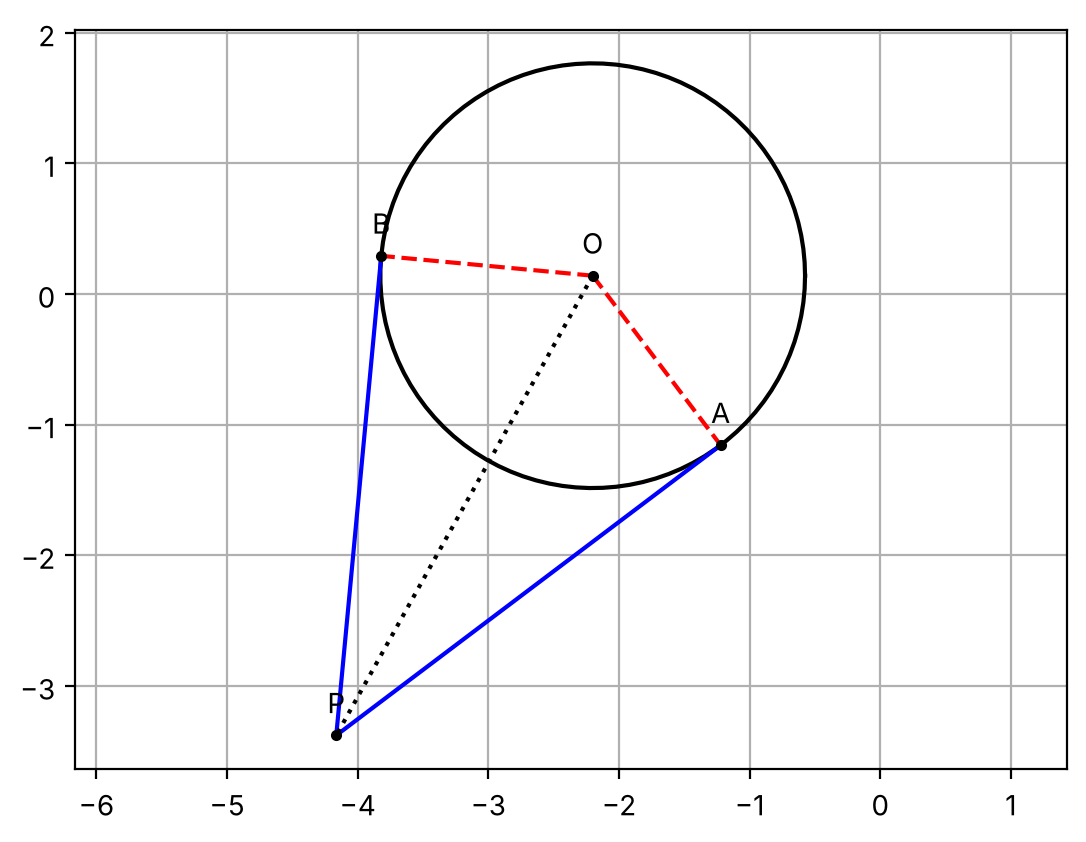
\includegraphics[width=0.70\linewidth]{figs/q33.png}
\caption{Equal tangent lengths $PA = PB$}
\label{fig:cb10-q33}
\end{figure}

\item Find the sum of first $16$ terms of an Arithmetic Progression whose $4^{\text{th}}$ and $9^{\text{th}}$ terms are $-15$ and $-30$ respectively.
\hfill (CBSE X 30/C/3, Q34)

\hfill OR \\
If the sum of first $14$ terms of an Arithmetic Progression is $1050$ and its fourth term is $40$, find its $20^{\text{th}}$ term.

\solution From \eqref{eq:cb10-ap-term}, $x(4) = a + 3d = -15$ and $x(9) = a + 8d = -30$,
\begin{align}
\myvec{1 & 3 & -15 \\ 1 & 8 & -30} \xrightarrow{R_2 \leftarrow R_2 - R_1} \myvec{1 & 3 & -15 \\ 0 & 5 & -15}
\implies d = -3, \quad a = -6
\end{align}
From \eqref{eq:cb10-ap-sum},
\begin{align}
S_{16} = \frac{16}{2}\brak{2\brak{-6} + 15\brak{-3}} = 8\brak{-57} = -456
\end{align}

\textbf{OR:} $S_{14} = 7\brak{2a + 13d} = 1050$ and $x(4) = a + 3d = 40$,
\begin{align}
\myvec{2 & 13 & 150 \\ 1 & 3 & 40} &\xrightarrow{R_1 \leftrightarrow R_2} \myvec{1 & 3 & 40 \\ 2 & 13 & 150} \xrightarrow{R_2 \leftarrow R_2 - 2R_1} \myvec{1 & 3 & 40 \\ 0 & 7 & 70} \\
&\implies d = 10, \quad a = 10
\end{align}
\begin{align}
x(20) = a + 19d = 10 + 190 = 200
\end{align}
The following code builds the AP with the unit step function \eqref{eq:cb10-step} and sums it with the window $u(n-1) - u(n-N-1)$ in \figref{fig:cb10-q34}.
\begin{lstlisting}[frame=single, basicstyle=\rmfamily, escapeinside={(*@}{@*)}]
(*@\makebox[\dimexpr\linewidth-2\fboxsep-2\fboxrule\relax][c]{codes/q34.py}@*)
\end{lstlisting}
\begin{figure}[H]
\centering
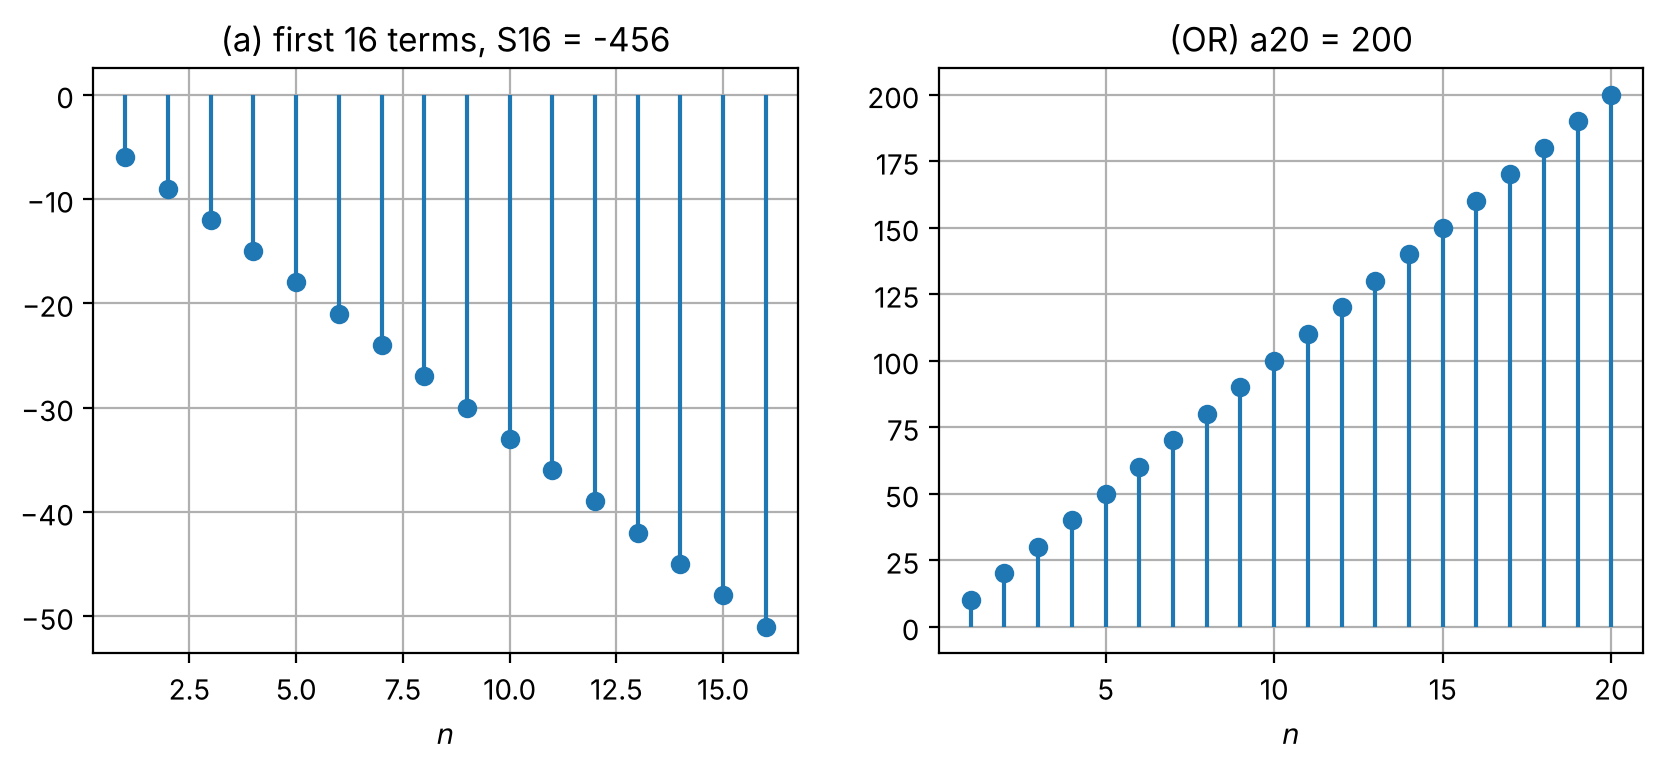
\includegraphics[width=0.85\linewidth]{figs/q34.png}
\caption{$S_{16} = -456$ and $x(20) = 200$}
\label{fig:cb10-q34}
\end{figure}

\item Sides $AB$ and $AC$ and median $AD$ of $\triangle ABC$ are respectively proportional to sides $PQ$ and $PR$ and median $PM$ of $\triangle PQR$. Show that $\triangle ABC \sim \triangle PQR$.
\hfill (CBSE X 30/C/3, Q35)

\hfill OR \\
In the figure, $BN$ and $CM$ are medians of a $\triangle ABC$ right-angled at $A$. Prove that $4\brak{BN^2 + CM^2} = 5BC^2$.

\solution Let $\dfrac{AB}{PQ} = \dfrac{AC}{PR} = \dfrac{AD}{PM} = k$. Extend $AD$ to $\vec{E} = 2\vec{D} - \vec{A}$ and $PM$ to $\vec{S} = 2\vec{M} - \vec{P}$. Since the diagonals $AE$ and $BC$ of $ABEC$ bisect each other, $ABEC$ is a parallelogram and $BE = AC$. Similarly $QS = PR$. Also $AE = 2AD$, $PS = 2PM$. Hence
\begin{align}
\frac{AB}{PQ} = \frac{BE}{QS} = \frac{AE}{PS} = k
\end{align}
and $\triangle ABE \sim \triangle PQS$ (SSS), so $\angle BAE = \angle QPS$. In the same way $\triangle ACE \sim \triangle PRS$ and $\angle CAE = \angle RPS$. Adding, $\angle BAC = \angle QPR$. Now $\frac{AB}{PQ} = \frac{AC}{PR}$ with the included angles equal gives $\triangle ABC \sim \triangle PQR$ (SAS). $\blacksquare$

\textbf{OR:} Take $\vec{A} = \vec{0}$, $\vec{B} = b\vec{e}_1$, $\vec{C} = c\vec{e}_2$. The mid points are $\vec{M} = \frac{b}{2}\vec{e}_1$ and $\vec{N} = \frac{c}{2}\vec{e}_2$. Then
\begin{align}
BN^2 &= \norm{\vec{B}-\vec{N}}^2 = b^2 + \frac{c^2}{4}, \quad CM^2 = \norm{\vec{C}-\vec{M}}^2 = c^2 + \frac{b^2}{4} \\
4\brak{BN^2 + CM^2} &= 4\cdot\frac{5}{4}\brak{b^2 + c^2} = 5\brak{b^2 + c^2} = 5BC^2
\end{align}
using \eqref{eq:cb10-pyth}. $\blacksquare$

The following code checks both parts numerically in \figref{fig:cb10-q35}: for an assumed triangle and $k = 2$ the sides, medians, angles and the identity are verified.
\begin{lstlisting}[frame=single, basicstyle=\rmfamily, escapeinside={(*@}{@*)}]
(*@\makebox[\dimexpr\linewidth-2\fboxsep-2\fboxrule\relax][c]{codes/q35.py}@*)
\end{lstlisting}
\begin{figure}[H]
\centering
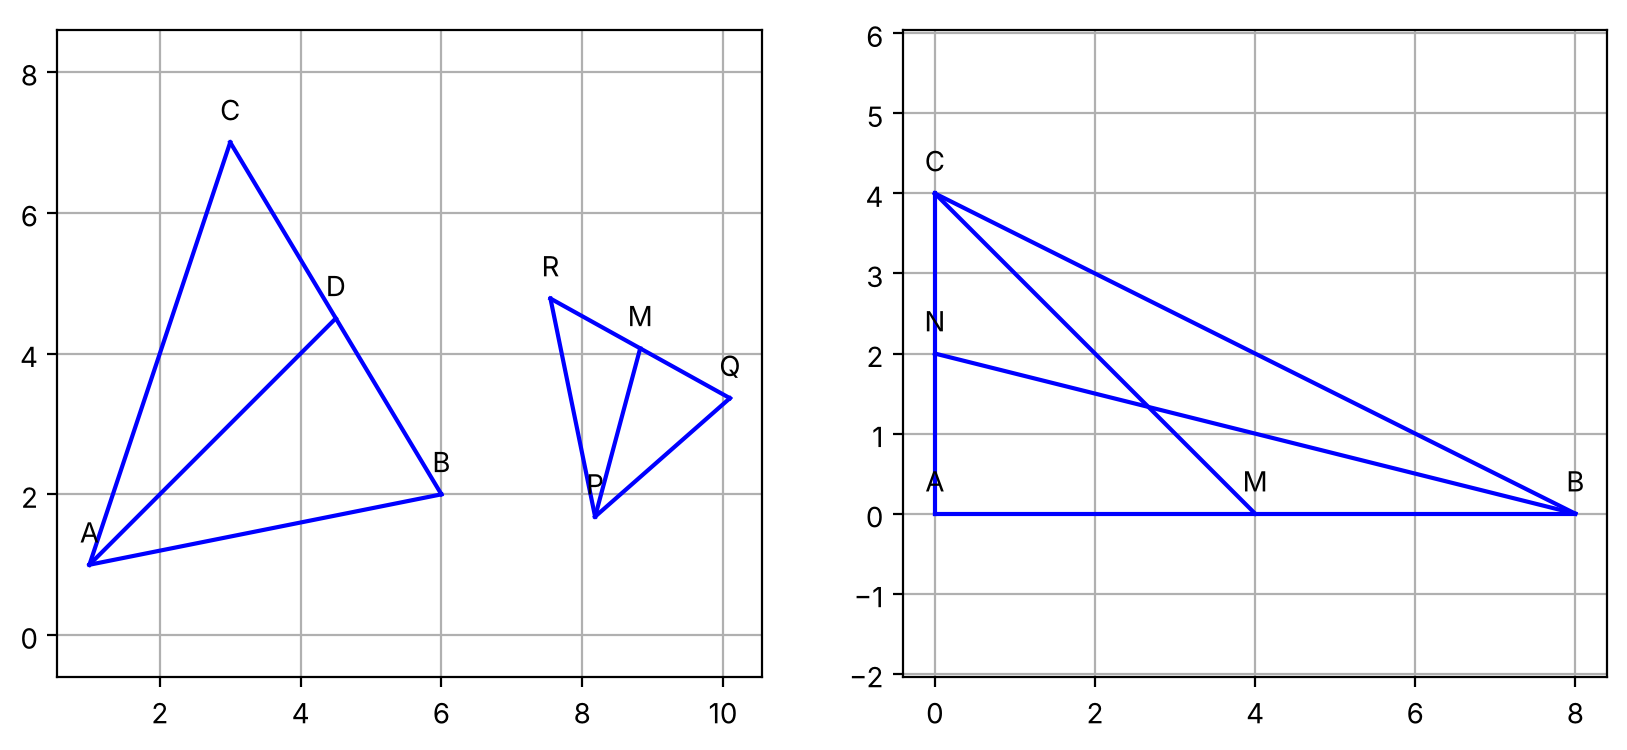
\includegraphics[width=0.85\linewidth]{figs/q35.png}
\caption{Similar triangles with medians (left) and the right triangle (right)}
\label{fig:cb10-q35}
\end{figure}

\item The angles of depression of the top and bottom of a tower as seen from the top of a $60\sqrt{3}$ m high cliff are $45^\circ$ and $60^\circ$ respectively. Find the height of the tower. (Use $\sqrt{3} = 1.73$)
\hfill (CBSE X 30/C/3, Q36)

\solution Let $\vec{F} = \vec{0}$ be the foot of the cliff and $\vec{C} = \myvec{0 \\ 60\sqrt{3}}$ its top. From \eqref{eq:cb10-depr}, the lines of sight are $\vec{x} = \vec{C} + \lambda\vec{d}\brak{\theta}$ with $\vec{d}\brak{60^\circ} = \myvec{\frac{1}{2} \\ -\frac{\sqrt{3}}{2}}$ and $\vec{d}\brak{45^\circ} = \myvec{\frac{1}{\sqrt{2}} \\ -\frac{1}{\sqrt{2}}}$.

The bottom $\vec{B}$ of the tower is where the first line meets the ground $\vec{e}_2^{\top}\vec{x} = 0$:
\begin{align}
\vec{n}_1 &= \vec{\Omega}\vec{d}\brak{60^\circ} = \myvec{-\frac{\sqrt{3}}{2} \\ -\frac{1}{2}} \\
\myvec{-\frac{\sqrt{3}}{2} & -\frac{1}{2} \\ 0 & 1}\vec{x} &= \myvec{\vec{n}_1^{\top}\vec{C} \\ 0} = \myvec{-30\sqrt{3} \\ 0}
\implies \vec{B} = \myvec{60 \\ 0}
\end{align}
The top $\vec{T}$ is where the $45^\circ$ line meets the vertical line $\vec{e}_1^{\top}\vec{x} = 60$:
\begin{align}
\myvec{-\frac{1}{\sqrt{2}} & -\frac{1}{\sqrt{2}} \\ 1 & 0}\vec{x} &= \myvec{-\frac{60\sqrt{3}}{\sqrt{2}} \\ 60} \\
\implies \vec{T} &= \myvec{60 \\ 60\sqrt{3} - 60}
\end{align}
(both systems solved by Gauss elimination). Hence the height of the tower is
\begin{align}
60\brak{\sqrt{3} - 1} = 60\brak{0.73} = 43.8 \text{ m}
\end{align}
The following code gives $43.92$ m with the exact $\sqrt{3}$ and $43.8$ m with $\sqrt{3} = 1.73$ in \figref{fig:cb10-q36}.
\begin{lstlisting}[frame=single, basicstyle=\rmfamily, escapeinside={(*@}{@*)}]
(*@\makebox[\dimexpr\linewidth-2\fboxsep-2\fboxrule\relax][c]{codes/q36.py}@*)
\end{lstlisting}
\begin{figure}[H]
\centering
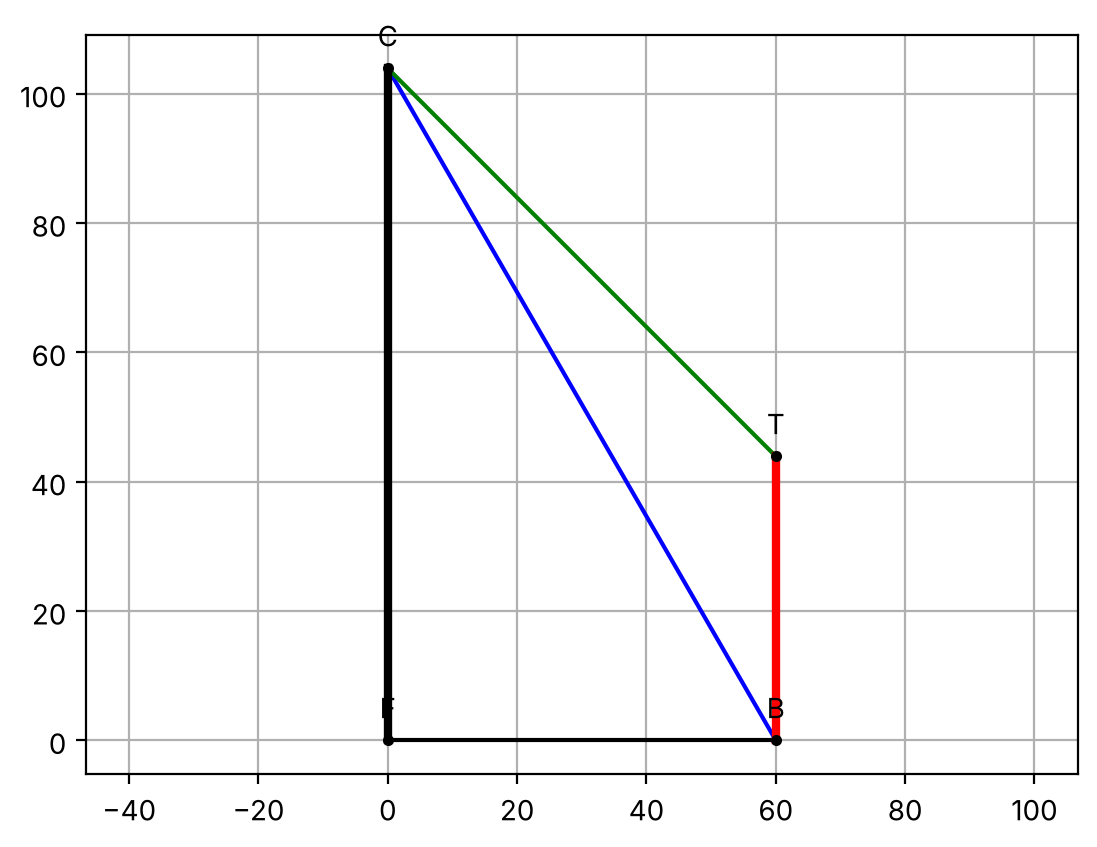
\includegraphics[width=0.50\linewidth]{figs/q36.png}
\caption{Cliff $FC$ and tower $BT$}
\label{fig:cb10-q36}
\end{figure}

\item $A$ and $B$ jointly finish a piece of work in $15$ days. When they work separately, $A$ takes $16$ days less than the number of days taken by $B$ to finish the same piece of work. Find the number of days taken by $B$ to finish the work.
\hfill (CBSE X 30/C/3, Q38)

\solution Let $A$ take $x$ days. Then $B$ takes $x + 16$ days. From \eqref{eq:cb10-work},
\begin{align}
\frac{1}{x} + \frac{1}{x+16} = \frac{1}{15} \implies f(x) = x^2 - 14x - 240 = 0
\end{align}
Applying the Newton-Raphson iteration \eqref{eq:cb10-nr},
\begin{align}
x_{n+1} = x_n - \frac{x_n^2 - 14x_n - 240}{2x_n - 14}
\end{align}
Starting from $x_0 = 30$: $x_1 = 24.7826$, $x_2 = 24.0172$, $x_3 = 24.000009$, $x_4 = 24.000000$. Starting from $x_0 = -20$ the iteration converges to $-10$, which is rejected since the number of days is positive. Therefore $A$ takes $24$ days and
\begin{align}
B = x + 16 = 40 \text{ days}
\end{align}
Check: $\frac{1}{24} + \frac{1}{40} = \frac{1}{15}$. The following C code gives this and draws \figref{fig:cb10-q38}.
\begin{lstlisting}[frame=single, basicstyle=\rmfamily, escapeinside={(*@}{@*)}]
(*@\makebox[\dimexpr\linewidth-2\fboxsep-2\fboxrule\relax][c]{codes/q38.c}@*)
\end{lstlisting}
\begin{figure}[H]
\centering
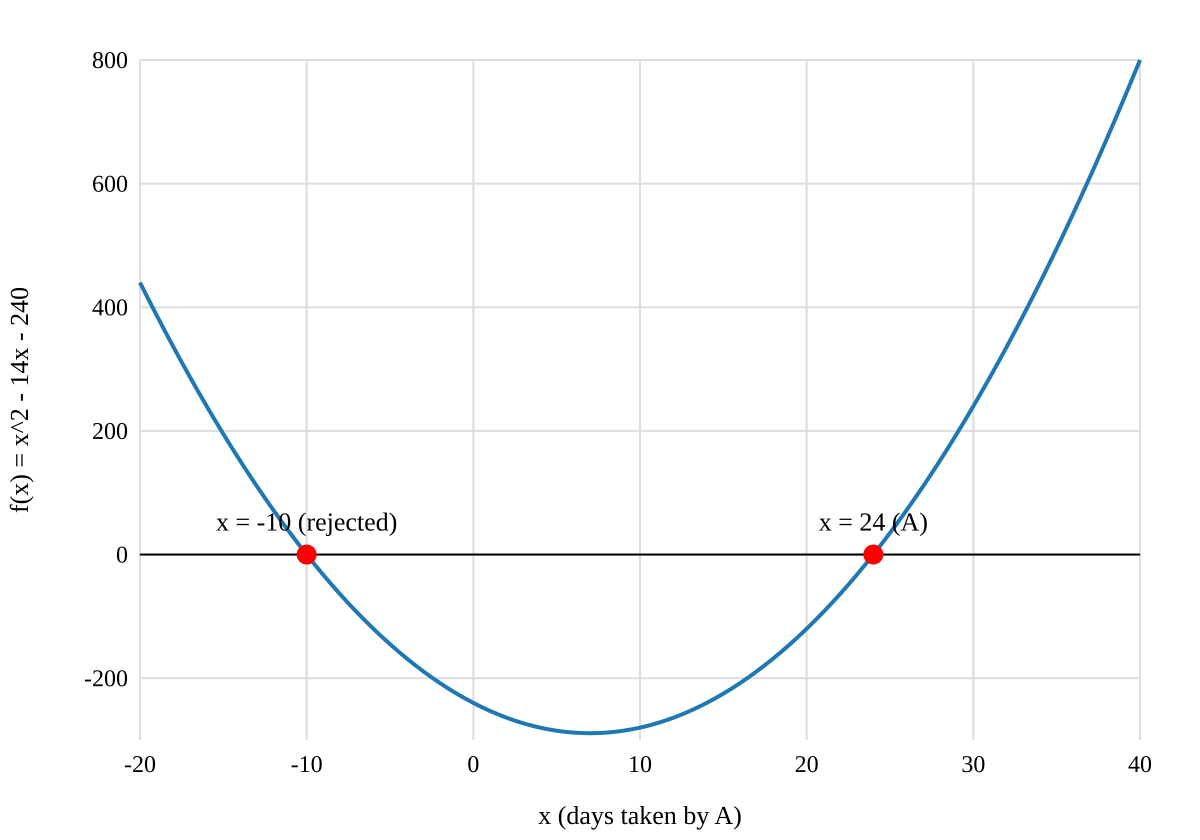
\includegraphics[width=0.55\linewidth]{figs/q38.png}
\caption{$f(x) = x^2 - 14x - 240$}
\label{fig:cb10-q38}
\end{figure}

\item If the polynomial $f(x) = 3x^4 - 9x^3 + x^2 + 15x + k$ is completely divisible by $3x^2 - 5$, then find the value of $k$. Using the quotient so obtained, find two zeroes of the polynomial.
\hfill (CBSE X 30/C/3, Q39)

\hfill OR \\
Find all the zeroes of the polynomial $x^4 - 8x^3 + 23x^2 - 28x + 12$ if two of its zeroes are $2$ and $3$.

\solution Dividing as in \eqref{eq:cb10-polydiv},
\begin{align}
3x^4 - 9x^3 + x^2 + 15x + k = \brak{3x^2 - 5}\brak{x^2 - 3x + 2} + \brak{k + 10}
\end{align}
For complete divisibility the remainder $k + 10 = 0$, so $k = -10$. The quotient is $q(x) = x^2 - 3x + 2$. Its zeroes from the Newton-Raphson iteration \eqref{eq:cb10-nr},
\begin{align}
x_{n+1} = x_n - \frac{x_n^2 - 3x_n + 2}{2x_n - 3}
\end{align}
are $1$ (from $x_0 = 0$) and $2$ (from $x_0 = 3$). So two zeroes of $f$ are $1$ and $2$ (the other two are $\pm\sqrt{\frac{5}{3}}$ from $3x^2 - 5 = 0$).

\textbf{OR:} Since $2, 3$ are zeroes, $g(x) = \brak{x-2}\brak{x-3} = x^2 - 5x + 6$ divides the polynomial and
\begin{align}
x^4 - 8x^3 + 23x^2 - 28x + 12 = \brak{x^2 - 5x + 6}\brak{x^2 - 3x + 2}
\end{align}
The zeroes of $x^2 - 3x + 2$ are $1, 2$. Hence all the zeroes are $1, 2, 2, 3$. The following code verifies both parts in \figref{fig:cb10-q39}.
\begin{lstlisting}[frame=single, basicstyle=\rmfamily, escapeinside={(*@}{@*)}]
(*@\makebox[\dimexpr\linewidth-2\fboxsep-2\fboxrule\relax][c]{codes/q39.py}@*)
\end{lstlisting}
\begin{figure}[H]
\centering
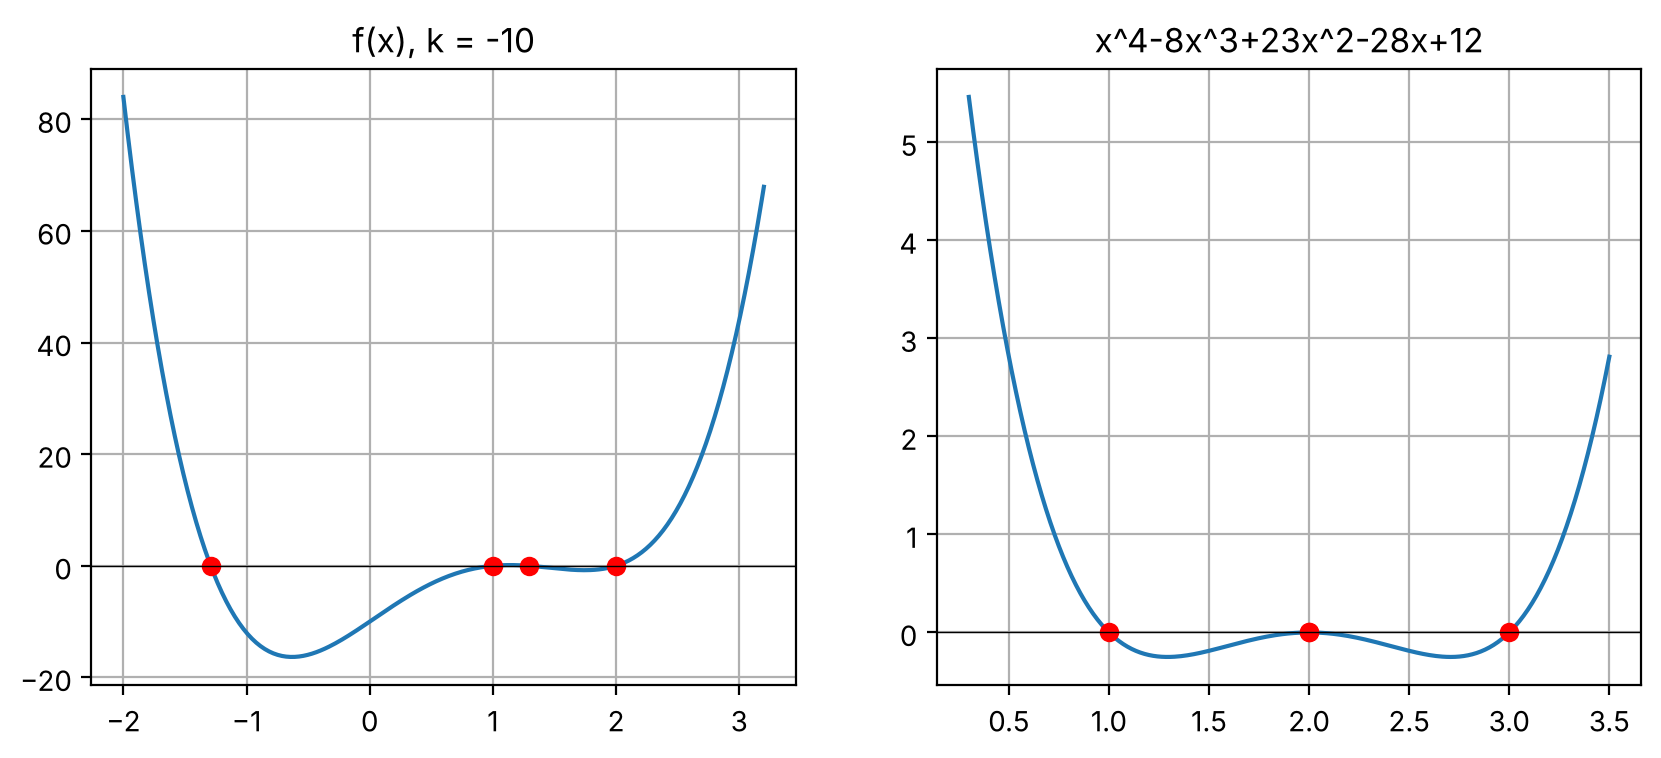
\includegraphics[width=0.85\linewidth]{figs/q39.png}
\caption{$f(x)$ for $k = -10$ (left) and the quartic of the OR part (right)}
\label{fig:cb10-q39}
\end{figure}

\item Draw `less than' ogive for the following distribution and hence find its median.
\begin{center}
\begin{tabular}{|c|c|c|c|c|c|c|c|}
\hline
Class & $20$--$30$ & $30$--$40$ & $40$--$50$ & $50$--$60$ & $60$--$70$ & $70$--$80$ & $80$--$90$ \\ \hline
Frequency & $10$ & $8$ & $12$ & $24$ & $6$ & $25$ & $15$ \\ \hline
\end{tabular}
\end{center}
\hfill (CBSE X 30/C/3, Q40)

\solution The cumulative frequencies (points of the `less than' ogive) are
\begin{center}
\begin{tabular}{|c|c|c|c|c|c|c|c|}
\hline
Less than & $30$ & $40$ & $50$ & $60$ & $70$ & $80$ & $90$ \\ \hline
$cf$ & $10$ & $18$ & $30$ & $54$ & $60$ & $85$ & $100$ \\ \hline
\end{tabular}
\end{center}
with $N = 100$, $\frac{N}{2} = 50$. The point of the ogive with ordinate $50$ lies on the segment from $\brak{50, 30}$ to $\brak{60, 54}$. On this segment $F(t) = 30 + 2.4\brak{t - 50}$ and the root of $F(t) - 50 = 0$ is found by the Newton-Raphson iteration \eqref{eq:cb10-nr} (one step since $F$ is linear):
\begin{align}
t = t_0 - \frac{F(t_0) - 50}{2.4} = 58.33
\end{align}
This agrees with \eqref{eq:cb10-median}:
\begin{align}
\text{median} = 50 + \frac{50 - 30}{24}\times 10 = 58.33
\end{align}
The following C code computes the ogive and the median and draws \figref{fig:cb10-q40}.
\begin{lstlisting}[frame=single, basicstyle=\rmfamily, escapeinside={(*@}{@*)}]
(*@\makebox[\dimexpr\linewidth-2\fboxsep-2\fboxrule\relax][c]{codes/q40.c}@*)
\end{lstlisting}
\begin{figure}[H]
\centering
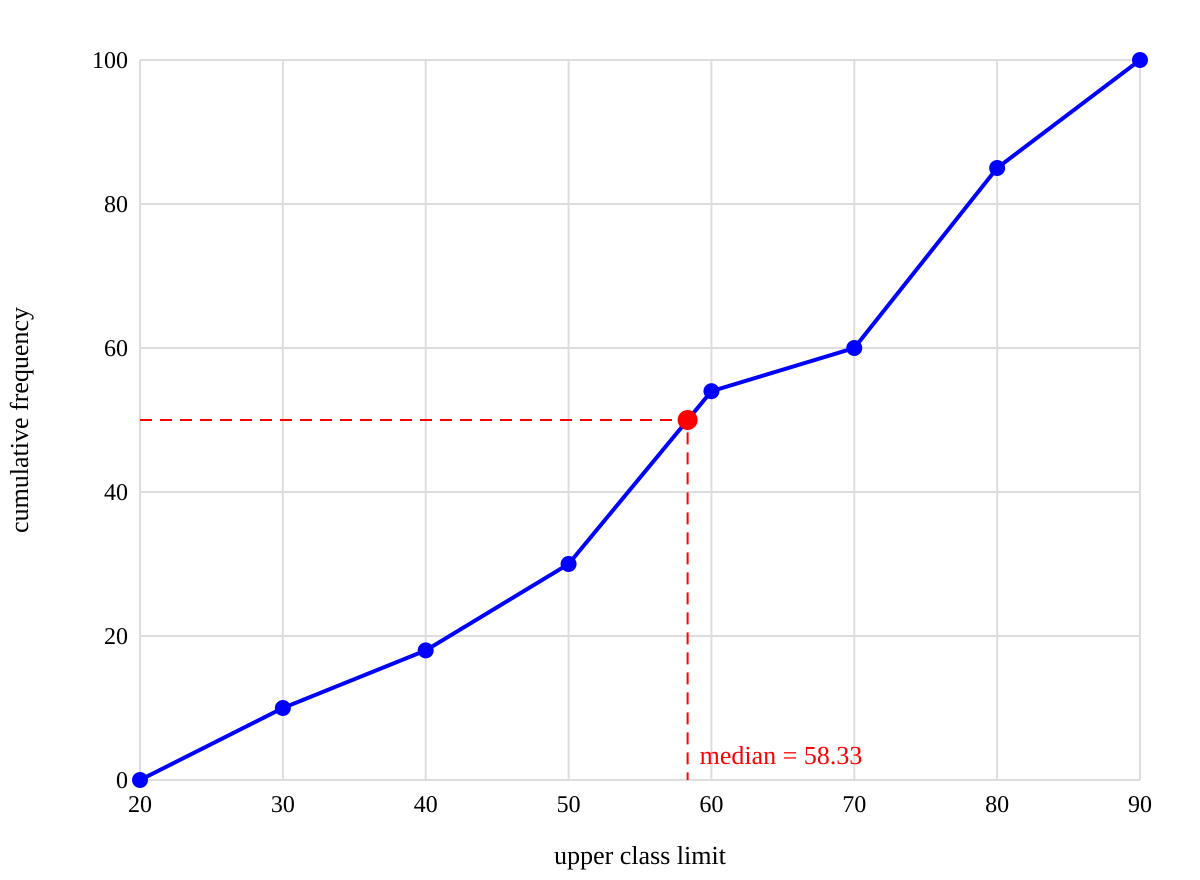
\includegraphics[width=0.70\linewidth]{figs/q40.png}
\caption{`Less than' ogive; median $= 58.33$}
\label{fig:cb10-q40}
\end{figure}

\end{enumerate}

\newpage

% ---------------- Class 12 ----------------
\graphicspath{{class12/}}
\section{CBSE Class 12 Mathematics 65/C/3}
\subsection{Formulae}
\begin{enumerate}[label=\thesubsection.\arabic*, ref=\thesubsection.\theenumi,itemsep=0pt]

\item The position vector of the point $\brak{x,y,z}$ is $\vec{a} = \myvec{x \\ y \\ z}$. The magnitude and dot product are
\begin{align}
\norm{\vec{a}} = \sqrt{\vec{a}^{\top}\vec{a}}, \quad \vec{a}^{\top}\vec{b} = \norm{\vec{a}}\norm{\vec{b}}\cos\theta
\label{eq:cb12-dot}
\end{align}
The vectors are perpendicular if $\vec{a}^{\top}\vec{b} = 0$.

\item The projection of $\vec{a}$ on $\vec{b}$ is
\begin{align}
\frac{\vec{a}^{\top}\vec{b}}{\norm{\vec{b}}}, \quad \frac{\text{proj. of } \vec{a} \text{ on } \vec{b}}{\text{proj. of } \vec{b} \text{ on } \vec{a}} = \frac{\norm{\vec{a}}}{\norm{\vec{b}}}
\label{eq:cb12-proj}
\end{align}

\item A plane is $\vec{n}^{\top}\vec{x} = c$. Two planes $\vec{n}_1^{\top}\vec{x} = c_1$, $\vec{n}_2^{\top}\vec{x} = c_2$ with $\vec{n}_1 = \lambda\vec{n}_2$ are parallel and their distance is
\begin{align}
d = \frac{\abs{c_1 - \lambda c_2}}{\norm{\vec{n}_1}}
\label{eq:cb12-planes}
\end{align}

\item The distance of the point $\vec{P}$ from the line through $\vec{A}$ with direction $\vec{e}$ ($\norm{\vec{e}} = 1$) is $\norm{\vec{P}-\vec{A} - \brak{\vec{e}^{\top}\brak{\vec{P}-\vec{A}}}\vec{e}}$. For the $x$-axis and $\vec{P} = \myvec{a \\ b \\ c}$ it is $\sqrt{b^2+c^2}$.
\label{eq:cb12-axis}

\item \textbf{Shortest distance between two lines} $\vec{x} = \vec{p}_1 + s\vec{d}_1$ and $\vec{x} = \vec{p}_2 + t\vec{d}_2$. Minimising $\norm{\vec{w} + s\vec{d}_1 - t\vec{d}_2}^2$, $\vec{w} = \vec{p}_1 - \vec{p}_2$, gives the normal equations
\begin{align}
\myvec{\vec{d}_1^{\top}\vec{d}_1 & -\vec{d}_1^{\top}\vec{d}_2 \\ \vec{d}_1^{\top}\vec{d}_2 & -\vec{d}_2^{\top}\vec{d}_2}\myvec{s \\ t} = -\myvec{\vec{d}_1^{\top}\vec{w} \\ \vec{d}_2^{\top}\vec{w}}
\label{eq:cb12-skew}
\end{align}
solved by Gauss elimination \eqref{eq:cb12-gauss}. The shortest distance is $\norm{\brak{\vec{p}_1 + s\vec{d}_1} - \brak{\vec{p}_2 + t\vec{d}_2}}$; the lines intersect iff it is $0$. No cross product is needed.

\item The planes through the intersection of $\vec{n}_1^{\top}\vec{x} = c_1$ and $\vec{n}_2^{\top}\vec{x} = c_2$ are
\begin{align}
\brak{\vec{n}_1 + \lambda\vec{n}_2}^{\top}\vec{x} = c_1 + \lambda c_2
\label{eq:cb12-family}
\end{align}
and the distance of $\vec{n}^{\top}\vec{x} = c$ from the origin is $\dfrac{\abs{c}}{\norm{\vec{n}}}$.

\item A vector perpendicular to $\vec{u}$ and $\vec{v}$ solves the homogeneous system $\vec{n}^{\top}\vec{u} = 0$, $\vec{n}^{\top}\vec{v} = 0$. Setting one component to $1$ and using Gauss elimination gives $\vec{n}$; the unit vector is $\pm\dfrac{\vec{n}}{\norm{\vec{n}}}$.
\label{eq:cb12-perp}

\item The area of the triangle with vertices $\vec{A}, \vec{B}, \vec{D}$ is
\begin{align}
\frac{1}{2}\abs{\vec{n}^{\top}\brak{\vec{D}-\vec{A}}}, \quad \vec{n} = \myvec{0 & 1 \\ -1 & 0}\brak{\vec{B}-\vec{A}}
\label{eq:cb12-area}
\end{align}
The line through $\vec{A}, \vec{B}$ is $\vec{n}^{\top}\vec{x} = \vec{n}^{\top}\vec{A}$.

\item The probability mass function (pmf) of a discrete random variable $X$ is $p_X(x) = \pr{X=x}$ with
\begin{align}
\sum_x p_X(x) = 1, \quad \pr{X \in E} = \sum_{x\in E}p_X(x), \quad \pr{E'} = 1 - \pr{E}
\label{eq:cb12-pmf}
\end{align}
For independent $A, B$ the joint pmf is the outer product $p_{AB} = p_A p_B^{\top}$ and for $S = X+Y$ the pmf is the convolution $p_S = p_X * p_Y$.

\item The conditional probability is
\begin{align}
\pr{A|B} = \frac{\pr{AB}}{\pr{B}}
\label{eq:cb12-cond}
\end{align}

\item \textbf{Determinants.} By cofactor expansion along the first row
\begin{align}
\mydet{a & b \\ c & d} = ad - bc, \quad \mydet{\vec{A}} = \sum_{j}\brak{-1}^{1+j}a_{1j}M_{1j}
\label{eq:cb12-det}
\end{align}
A square matrix is singular iff $\mydet{\vec{A}} = 0$, and $\mydet{\vec{A}\vec{B}} = \mydet{\vec{A}}\mydet{\vec{B}}$. Row operations $R_i \leftarrow R_i + cR_j$ leave the determinant unchanged. Determinants are used only to evaluate $\mydet{\vec{A}}$, never to solve linear equations.

\item \textbf{Laplace transform.} For $t \ge 0$,
\begin{align}
F(s) = \int_0^{\infty} e^{-st}f(t)\,dt, \quad L\{1\} = \frac{1}{s},\ L\{t\} = \frac{1}{s^2},\ L\{e^{at}\} = \frac{1}{s-a}
\label{eq:cb12-laplace}
\end{align}
The differentiation properties are
\begin{align}
L\{f'\}(s) &= sF(s) - f(0) \label{eq:cb12-lap1}\\
L\{f''\}(s) &= s^2F(s) - sf(0) - f'(0) \label{eq:cb12-lap2}
\end{align}
\solution Integrating by parts, $\int_0^\infty e^{-st}f'(t)\,dt = \left[e^{-st}f(t)\right]_0^\infty + s\int_0^\infty e^{-st}f(t)\,dt = -f(0) + sF(s)$. Applying this twice gives \eqref{eq:cb12-lap2}. On a finite interval $[0,T]$ the extra term $e^{-sT}f(T)$ appears. In the codes $F(s)$ is evaluated numerically with the trapezoidal rule \eqref{eq:cb12-trap}.

\item \textbf{Euler forward difference.} For small $h$,
\begin{align}
f'(x) \approx \frac{f(x+h) - f(x)}{h}, \quad f''(x) \approx \frac{f(x+2h) - 2f(x+h) + f(x)}{h^2}
\label{eq:cb12-euler-diff}
\end{align}
For $\frac{dy}{dx} = F(x,y)$, $y(x_0) = y_0$, the Euler forward method is
\begin{align}
y_{n+1} = y_n + hF\brak{x_n, y_n}
\label{eq:cb12-euler}
\end{align}

\item \textbf{Linear differential equations.} The equation $\frac{dy}{dx} + P(x)y = Q(x)$ has integrating factor $e^{\int P\,dx}$. With the substitution $x = e^t$, $x\frac{dy}{dx} = \frac{dy}{dt}$ and equations of the form $x\frac{dy}{dx} = \alpha y + g(x)$ become constant coefficient equations that are solved by the Laplace transform \eqref{eq:cb12-lap1}.
\label{eq:cb12-linode}

\item \textbf{Trapezoidal rule.} For $N$ sub-intervals of width $h = \dfrac{b-a}{N}$,
\begin{align}
\int_a^b f(x)\,dx \approx \frac{h}{2}\sbrak{f(x_0) + 2\sum_{i=1}^{N-1}f(x_i) + f(x_N)}
\label{eq:cb12-trap}
\end{align}
The limit of sums is $\int_a^b f(x)\,dx = \lim_{N\to\infty}h\sum_{i=1}^{N}f\brak{a + ih}$.

\item \textbf{Newton-Raphson method.} A root of $f(x) = 0$ is obtained from
\begin{align}
x_{n+1} = x_n - \frac{f\brak{x_n}}{f'\brak{x_n}}
\label{eq:cb12-nr}
\end{align}

\item \textbf{Gauss elimination.} The system $\vec{A}\vec{x} = \vec{b}$ is reduced by row operations
\begin{align}
\myvec{\vec{A} & \vec{b}} \xrightarrow{\text{row operations}} \myvec{\vec{U} & \vec{c}}
\label{eq:cb12-gauss}
\end{align}
with $\vec{U}$ upper triangular, and solved by back substitution.

\end{enumerate}

\newpage
\subsection{Problems}
\begin{enumerate}[label=\thesubsection.\arabic*, ref=\thesubsection.\theenumi,itemsep=0pt]

\item If $\vec{a}, \vec{b}, \vec{c}$ are the position vectors of the points $A\brak{2,3,-4}$, $B\brak{3,-4,-5}$ and $C\brak{3,2,-3}$ respectively, then $\norm{\vec{a}+\vec{b}+\vec{c}}$ is equal to
\hfill (CBSE XII 65/C/3, Q1)
\begin{enumerate}[itemsep=0pt]
\begin{multicols}{4}
\item $\sqrt{113}$
\item $\sqrt{185}$
\item $\sqrt{203}$
\item $\sqrt{209}$
\end{multicols}
\end{enumerate}

\solution
\begin{align}
\vec{a}+\vec{b}+\vec{c} = \myvec{2 \\ 3 \\ -4} + \myvec{3 \\ -4 \\ -5} + \myvec{3 \\ 2 \\ -3} = \myvec{8 \\ 1 \\ -12}
\end{align}
From \eqref{eq:cb12-dot}, $\norm{\vec{a}+\vec{b}+\vec{c}}^2 = 64 + 1 + 144 = 209$. Hence option (D). The following code verifies this.
\begin{lstlisting}[frame=single, basicstyle=\rmfamily, escapeinside={(*@}{@*)}]
(*@\makebox[\dimexpr\linewidth-2\fboxsep-2\fboxrule\relax][c]{codes/q1.py}@*)
\end{lstlisting}

\item The distance between the planes $4x - 4y + 2z + 5 = 0$ and $2x - 2y + z + 6 = 0$ is
\hfill (CBSE XII 65/C/3, Q3)
\begin{enumerate}[itemsep=0pt]
\begin{multicols}{4}
\item $\frac{1}{6}$
\item $\frac{7}{6}$
\item $\frac{11}{6}$
\item $\frac{16}{6}$
\end{multicols}
\end{enumerate}

\solution In the form $\vec{n}^{\top}\vec{x} = c$: $\vec{n}_1 = \myvec{4 \\ -4 \\ 2}$, $c_1 = -5$ and $\vec{n}_2 = \myvec{2 \\ -2 \\ 1}$, $c_2 = -6$. Since $\vec{n}_1 = 2\vec{n}_2$ the planes are parallel. From \eqref{eq:cb12-planes} with $\lambda = 2$,
\begin{align}
d = \frac{\abs{-5 - 2\brak{-6}}}{\norm{\vec{n}_1}} = \frac{7}{\sqrt{16+16+4}} = \frac{7}{6}
\end{align}
Hence option (B). The following code verifies this.
\begin{lstlisting}[frame=single, basicstyle=\rmfamily, escapeinside={(*@}{@*)}]
(*@\makebox[\dimexpr\linewidth-2\fboxsep-2\fboxrule\relax][c]{codes/q3.py}@*)
\end{lstlisting}

\item The probabilities of solving a specific question independently by $A$ and $B$ are $\frac{1}{3}$ and $\frac{1}{5}$ respectively. If both try to solve the question independently, the probability that the question is solved is
\hfill (CBSE XII 65/C/3, Q4)
\begin{enumerate}[itemsep=0pt]
\begin{multicols}{4}
\item $\frac{7}{15}$
\item $\frac{8}{15}$
\item $\frac{2}{15}$
\item $\frac{14}{15}$
\end{multicols}
\end{enumerate}

\solution The pmfs of $A$ and $B$ (index $0$: fails, $1$: solves) are $p_A = \myvec{\frac{2}{3} \\ \frac{1}{3}}$, $p_B = \myvec{\frac{4}{5} \\ \frac{1}{5}}$. By independence, from \eqref{eq:cb12-pmf} the joint pmf is
\begin{align}
p_{AB} = p_Ap_B^{\top} = \myvec{\frac{8}{15} & \frac{2}{15} \\ \frac{4}{15} & \frac{1}{15}}
\end{align}
The question is solved unless both fail, so $\pr{\text{solved}} = 1 - \frac{8}{15} = \frac{7}{15}$. Hence option (A). The following code verifies this.
\begin{lstlisting}[frame=single, basicstyle=\rmfamily, escapeinside={(*@}{@*)}]
(*@\makebox[\dimexpr\linewidth-2\fboxsep-2\fboxrule\relax][c]{codes/q4.py}@*)
\end{lstlisting}

\item If $\sec^{-1}\brak{\dfrac{1+x}{1-y}} = a$, then $\dfrac{dy}{dx}$ is equal to
\hfill (CBSE XII 65/C/3, Q6)
\begin{enumerate}[itemsep=0pt]
\begin{multicols}{4}
\item $\frac{x-1}{y-1}$
\item $\frac{x-1}{y+1}$
\item $\frac{y-1}{x+1}$
\item $\frac{y+1}{x-1}$
\end{multicols}
\end{enumerate}

\solution Let $k = \sec a$ (a constant). Then $\frac{1+x}{1-y} = k$, i.e.
\begin{align}
y = 1 - \frac{1+x}{k}
\end{align}
Take $x \to t$. By \eqref{eq:cb12-laplace},
\begin{align}
Y(s) = \frac{1}{s} - \frac{1}{k}\brak{\frac{1}{s^2} + \frac{1}{s}}, \quad y(0) = 1 - \frac{1}{k}
\end{align}
From \eqref{eq:cb12-lap1},
\begin{align}
L\{y'\}(s) &= sY(s) - y(0) = 1 - \frac{1}{ks} - \frac{1}{k} - 1 + \frac{1}{k} = -\frac{1}{k}\cdot\frac{1}{s} = L\cbrak{-\frac{1}{k}} \\
\implies \frac{dy}{dx} &= -\frac{1}{k} = -\frac{1-y}{1+x} = \frac{y-1}{x+1}
\end{align}
Hence option (C). The following code checks the Laplace relation numerically with $a = 1$ rad (assumed), the Euler forward difference \eqref{eq:cb12-euler-diff} and the four options.
\begin{lstlisting}[frame=single, basicstyle=\rmfamily, escapeinside={(*@}{@*)}]
(*@\makebox[\dimexpr\linewidth-2\fboxsep-2\fboxrule\relax][c]{codes/q6.py}@*)
\end{lstlisting}

\item $\displaystyle\int_0^1 \tan\brak{\sin^{-1}x}\,dx$ equals
\hfill (CBSE XII 65/C/3, Q9)
\begin{enumerate}[itemsep=0pt]
\begin{multicols}{4}
\item 2
\item 0
\item $-1$
\item 1
\end{multicols}
\end{enumerate}

\solution Put $x = \sin\theta$, $dx = \cos\theta\,d\theta$, $\theta \in \sbrak{0, \frac{\pi}{2}}$. Then $\tan\theta\cos\theta = \sin\theta$ and
\begin{align}
\int_0^1 \tan\brak{\sin^{-1}x}\,dx = \int_0^{\pi/2}\sin\theta\,d\theta
\end{align}
The trapezoidal rule \eqref{eq:cb12-trap} gives $0.99794$ for $N = 10$, $0.99998$ for $N = 100$ and $1.00000$ for $N = 10^4$, so the value is $1$ (exactly $\sbrak{-\cos\theta}_0^{\pi/2} = 1$). Hence option (D). The following code verifies this.
\begin{lstlisting}[frame=single, basicstyle=\rmfamily, escapeinside={(*@}{@*)}]
(*@\makebox[\dimexpr\linewidth-2\fboxsep-2\fboxrule\relax][c]{codes/q9.py}@*)
\end{lstlisting}

\item The roots of the equation $\mydet{x & 0 & 8 \\ 4 & 1 & 3 \\ 2 & 0 & x} = 0$ are
\hfill (CBSE XII 65/C/3, Q10)
\begin{enumerate}[itemsep=0pt]
\begin{multicols}{4}
\item $-4, 4$
\item $2, -4$
\item $2, 4$
\item $2, 8$
\end{multicols}
\end{enumerate}

\solution Expanding along the second column, which has a single non-zero entry,
\begin{align}
\mydet{x & 0 & 8 \\ 4 & 1 & 3 \\ 2 & 0 & x} = 1\cdot\mydet{x & 8 \\ 2 & x} = x^2 - 16 = 0
\end{align}
The roots are found by the Newton-Raphson iteration \eqref{eq:cb12-nr}
\begin{align}
x_{n+1} = x_n - \frac{x_n^2 - 16}{2x_n} = \frac{1}{2}\brak{x_n + \frac{16}{x_n}}
\end{align}
which converges to $4$ from $x_0 = 5$ and to $-4$ from $x_0 = -5$. Hence option (A). The following code evaluates the determinant by cofactor expansion and finds the roots.
\begin{lstlisting}[frame=single, basicstyle=\rmfamily, escapeinside={(*@}{@*)}]
(*@\makebox[\dimexpr\linewidth-2\fboxsep-2\fboxrule\relax][c]{codes/q10.py}@*)
\end{lstlisting}

\item A square matrix $\vec{A}$ is said to be singular if \underline{\hspace{1.5cm}}.
\hfill (CBSE XII 65/C/3, Q11)

\hfill OR \\
If $\vec{A} = \myvec{3 & -5 \\ 2 & 0}$ and $\vec{B} = \myvec{1 & 17 \\ 0 & -10}$, then $\mydet{\vec{A}\vec{B}} = $ \underline{\hspace{1.5cm}}.

\solution From \eqref{eq:cb12-det}, $\vec{A}$ is singular if $\mydet{\vec{A}} = 0$. 

\textbf{OR:} $\mydet{\vec{A}} = 0 - \brak{-10} = 10$, $\mydet{\vec{B}} = -10$, so
\begin{align}
\mydet{\vec{A}\vec{B}} = \mydet{\vec{A}}\mydet{\vec{B}} = -100
\end{align}
(directly, $\vec{A}\vec{B} = \myvec{3 & 101 \\ 2 & 34}$ and $3\cdot 34 - 101\cdot 2 = -100$). The following code verifies this.
\begin{lstlisting}[frame=single, basicstyle=\rmfamily, escapeinside={(*@}{@*)}]
(*@\makebox[\dimexpr\linewidth-2\fboxsep-2\fboxrule\relax][c]{codes/q11.py}@*)
\end{lstlisting}

\item A card is picked at random from a pack of $52$ playing cards. Given that the picked up card is a queen, the probability of it being a queen of spades is \underline{\hspace{1.5cm}}.
\hfill (CBSE XII 65/C/3, Q13)

\solution Each card has pmf $\frac{1}{52}$. Let $Q$ be the event that the card is a queen and $QS$ the queen of spades. $\pr{Q} = \frac{4}{52}$, $\pr{QS\,Q} = \frac{1}{52}$. From \eqref{eq:cb12-cond},
\begin{align}
\pr{QS|Q} = \frac{1/52}{4/52} = \frac{1}{4}
\end{align}
Given a queen, the four queens are equally likely. The following code verifies this.
\begin{lstlisting}[frame=single, basicstyle=\rmfamily, escapeinside={(*@}{@*)}]
(*@\makebox[\dimexpr\linewidth-2\fboxsep-2\fboxrule\relax][c]{codes/q13.py}@*)
\end{lstlisting}

\item The integrating factor of the differential equation $x\dfrac{dy}{dx} - y = \log x$ is \underline{\hspace{1.5cm}}.
\hfill (CBSE XII 65/C/3, Q14)

\solution In the standard form $\frac{dy}{dx} - \frac{1}{x}y = \frac{\log x}{x}$, so from \ref{eq:cb12-linode},
\begin{align}
\text{IF} = e^{-\int \frac{dx}{x}} = \frac{1}{x}
\end{align}
\textbf{Laplace transform:} put $x = e^t$. Then $x\frac{dy}{dx} = \frac{dy}{dt}$ and the equation becomes $\frac{dy}{dt} - y = t$. From \eqref{eq:cb12-lap1} and \eqref{eq:cb12-laplace},
\begin{align}
sY - y_0 - Y = \frac{1}{s^2} \implies Y(s) = \frac{y_0}{s-1} + \frac{1}{s^2\brak{s-1}}
\end{align}
Here the integrating factor in $t$ is $e^{-t} = \frac{1}{x}$, and the solution is $y = -\brak{\log x + 1} + Cx$ with $C = y_0 + 1$. The IF makes the left side exact, $\frac{d}{dx}\brak{\frac{y}{x}} = \frac{xy' - y}{x^2} = \frac{\log x}{x^2}$, which the code checks with the Euler forward difference \eqref{eq:cb12-euler-diff}. The code also compares the numerical Laplace transform of $y(t)$ with $Y(s)$ and solves the ODE by the Euler forward method \eqref{eq:cb12-euler} in \figref{fig:cb12-q14}.
\begin{lstlisting}[frame=single, basicstyle=\rmfamily, escapeinside={(*@}{@*)}]
(*@\makebox[\dimexpr\linewidth-2\fboxsep-2\fboxrule\relax][c]{codes/q14.py}@*)
\end{lstlisting}
\begin{figure}[H]
\centering
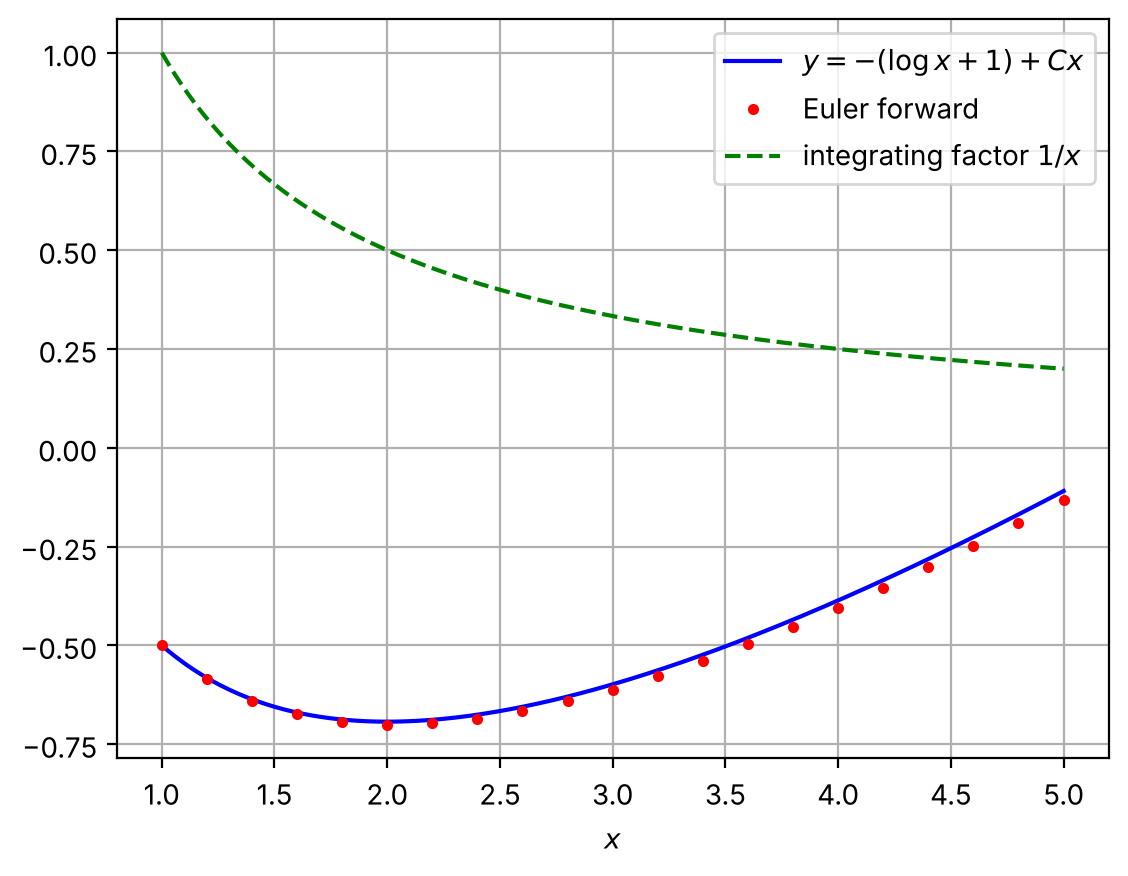
\includegraphics[width=0.65\linewidth]{figs/q14.png}
\caption{Solution, Euler forward method and the integrating factor $1/x$}
\label{fig:cb12-q14}
\end{figure}

\item If $y = \log x$, then $\dfrac{d^2y}{dx^2} = $ \underline{\hspace{1.5cm}}.
\hfill (CBSE XII 65/C/3, Q15)

\solution $y' = \frac{1}{x}$ and $y'' = -\frac{1}{x^2}$. 

\textbf{Laplace transform:} with $t = x - 1$, $y\brak{t} = \log\brak{1+t}$, $y(0) = 0$, $y'(0) = 1$. From \eqref{eq:cb12-lap1} and \eqref{eq:cb12-lap2},
\begin{align}
L\{y'\} = sY(s), \quad L\{y''\} = s^2Y(s) - 1
\end{align}
The code computes $Y(s)$ with the trapezoidal rule and finds, e.g. at $s = 2$, $L\{y'\} = 0.361329$ against $sY = 0.361329$ for $y' = \frac{1}{1+t}$, and $L\{y''\} = -0.277343$ against $s^2Y - 1 = -0.277343$ for $y'' = -\frac{1}{\brak{1+t}^2}$. The Euler second difference \eqref{eq:cb12-euler-diff} gives $-0.9998, -0.2500, -0.0625$ at $x = 1, 2, 4$ which are $-\frac{1}{x^2}$. Hence
\begin{align}
\frac{d^2y}{dx^2} = -\frac{1}{x^2}
\end{align}
See \figref{fig:cb12-q15}.
\begin{lstlisting}[frame=single, basicstyle=\rmfamily, escapeinside={(*@}{@*)}]
(*@\makebox[\dimexpr\linewidth-2\fboxsep-2\fboxrule\relax][c]{codes/q15.py}@*)
\end{lstlisting}
\begin{figure}[H]
\centering
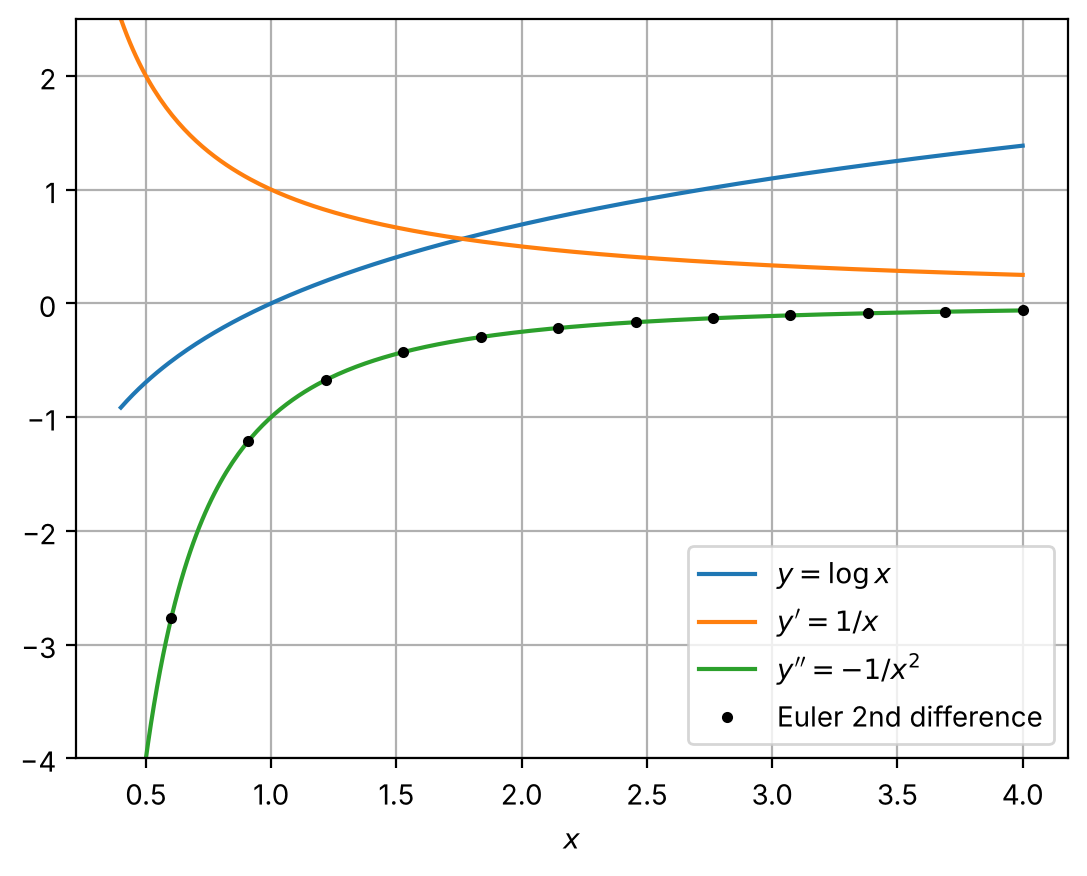
\includegraphics[width=0.65\linewidth]{figs/q15.png}
\caption{$y$, $y'$, $y''$ and the Euler second difference}
\label{fig:cb12-q15}
\end{figure}

\item Find the solution of the differential equation $\log\brak{\dfrac{dy}{dx}} = ax + by$.
\hfill (CBSE XII 65/C/3, Q17)

\solution $\frac{dy}{dx} = e^{ax}e^{by}$. Separating the variables,
\begin{align}
e^{-by}\,dy = e^{ax}\,dx \implies \frac{e^{ax}}{a} + \frac{e^{-by}}{b} = C
\end{align}
The equation is non-linear, so it is checked numerically. With $a = b = 1$ and $y(0) = 0$ (assumed) the solution is $e^x + e^{-y} = 2$, i.e. $y = -\log\brak{2 - e^x}$. The Euler forward method \eqref{eq:cb12-euler} with $500$ steps gives $y(0.5) = 1.0432$ against the exact $1.0462$. The Laplace derivative property \eqref{eq:cb12-lap1} on $[0, 0.5]$ is verified, $L\{e^{x+y}\} = sY - y(0) + e^{-sT}y(T)$, e.g. $0.583278$ at $s = 2$ on both sides. See \figref{fig:cb12-q17}.
\begin{lstlisting}[frame=single, basicstyle=\rmfamily, escapeinside={(*@}{@*)}]
(*@\makebox[\dimexpr\linewidth-2\fboxsep-2\fboxrule\relax][c]{codes/q17.py}@*)
\end{lstlisting}
\begin{figure}[H]
\centering
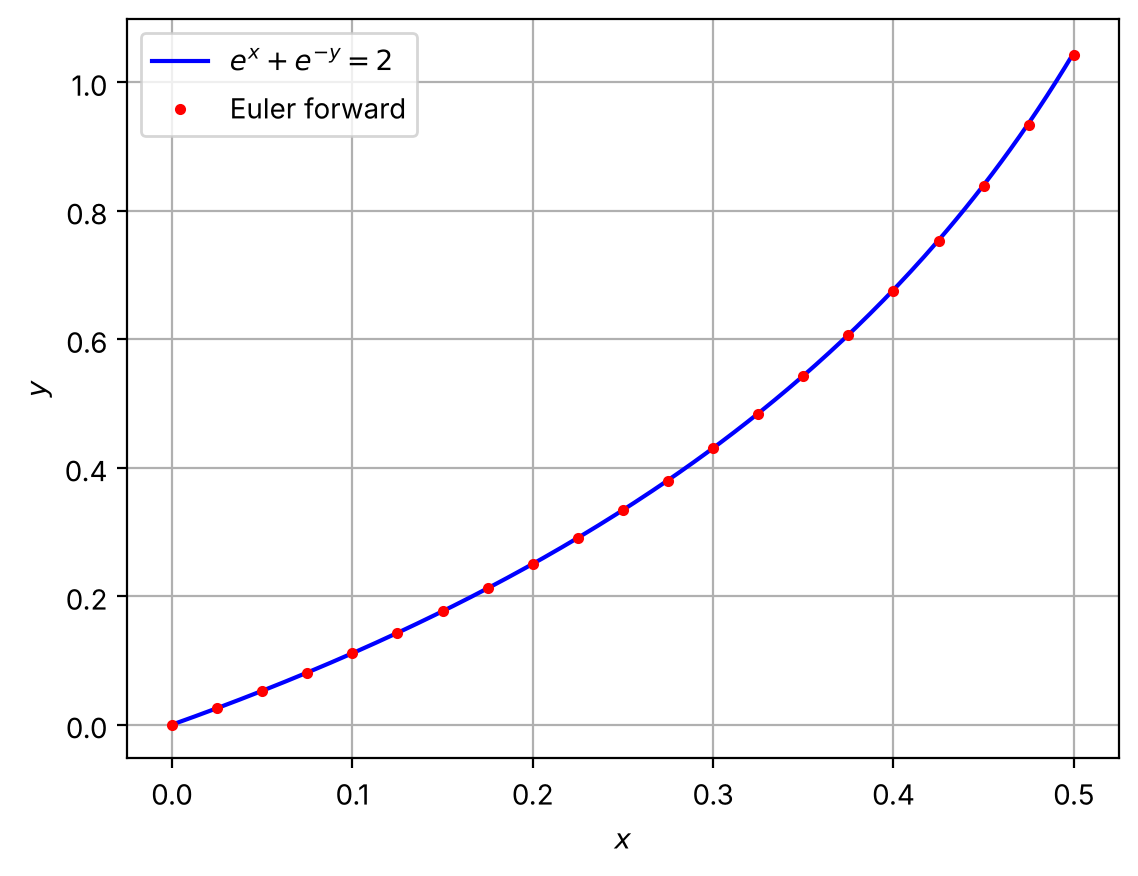
\includegraphics[width=0.55\linewidth]{figs/q17.png}
\caption{$e^x + e^{-y} = 2$ and the Euler forward method}
\label{fig:cb12-q17}
\end{figure}

\item If $\vec{a} = 2\hat{i} - \hat{j} + 2\hat{k}$ and $\vec{b} = 5\hat{i} - 3\hat{j} - 4\hat{k}$, then find the ratio $\dfrac{\text{projection of } \vec{a} \text{ on } \vec{b}}{\text{projection of } \vec{b} \text{ on } \vec{a}}$.
\hfill (CBSE XII 65/C/3, Q18)

\hfill OR \\
Let $\hat{a}$ and $\hat{b}$ be two unit vectors. If the vectors $\vec{c} = \hat{a} + 2\hat{b}$ and $\vec{d} = 5\hat{a} - 4\hat{b}$ are perpendicular to each other, then find the angle between $\hat{a}$ and $\hat{b}$.

\solution $\vec{a}^{\top}\vec{b} = 10 + 3 - 8 = 5$, $\norm{\vec{a}} = 3$, $\norm{\vec{b}} = \sqrt{50}$. From \eqref{eq:cb12-proj},
\begin{align}
\frac{\norm{\vec{a}}}{\norm{\vec{b}}} = \frac{3}{5\sqrt{2}}
\end{align}
\textbf{OR:} From \eqref{eq:cb12-dot}, $\vec{c}^{\top}\vec{d} = 5 - 4\cos\theta + 10\cos\theta - 8 = 6\cos\theta - 3 = 0$. Newton-Raphson \eqref{eq:cb12-nr} on $f\brak{\theta} = 6\cos\theta - 3$,
\begin{align}
\theta_{n+1} = \theta_n + \frac{6\cos\theta_n - 3}{6\sin\theta_n}
\end{align}
converges to $\theta = 60^\circ$. The following code verifies both parts.
\begin{lstlisting}[frame=single, basicstyle=\rmfamily, escapeinside={(*@}{@*)}]
(*@\makebox[\dimexpr\linewidth-2\fboxsep-2\fboxrule\relax][c]{codes/q18.py}@*)
\end{lstlisting}

\item Find the distance of the point $\brak{a,b,c}$ from the $x$-axis.
\hfill (CBSE XII 65/C/3, Q20)

\solution Let $\vec{P} = \myvec{a \\ b \\ c}$ and $\vec{e}_1 = \myvec{1 \\ 0 \\ 0}$. The foot of the perpendicular is $\brak{\vec{e}_1^{\top}\vec{P}}\vec{e}_1 = \myvec{a \\ 0 \\ 0}$ and from \ref{eq:cb12-axis},
\begin{align}
d = \norm{\vec{P} - a\vec{e}_1} = \norm{\myvec{0 \\ b \\ c}} = \sqrt{b^2 + c^2}
\end{align}
The following code verifies this for assumed points.
\begin{lstlisting}[frame=single, basicstyle=\rmfamily, escapeinside={(*@}{@*)}]
(*@\makebox[\dimexpr\linewidth-2\fboxsep-2\fboxrule\relax][c]{codes/q20.py}@*)
\end{lstlisting}

\item If $y = \sqrt{a + \sqrt{a + x}}$, then find $\dfrac{dy}{dx}$.
\hfill (CBSE XII 65/C/3, Q21)

\solution By the chain rule,
\begin{align}
\frac{dy}{dx} = \frac{1}{2\sqrt{a+\sqrt{a+x}}}\cdot\frac{1}{2\sqrt{a+x}} = \frac{1}{4\sqrt{a+x}\sqrt{a+\sqrt{a+x}}}
\end{align}
\textbf{Laplace transform:} with $a = 1$ (assumed) and $x \to t$, the property \eqref{eq:cb12-lap1} gives $L\{y'\} = sY(s) - y(0)$, $y(0) = \sqrt{2}$. The code computes $Y(s)$ by the trapezoidal rule: at $s = 2$, $L\{y'\} = 0.071386$ with $y'$ from the formula and $sY - y(0) = 0.071386$. The Euler forward difference \eqref{eq:cb12-euler-diff} gives $0.136853, 0.087324, 0.054952$ at $x = 0.5, 2, 5$, equal to the formula.
\begin{lstlisting}[frame=single, basicstyle=\rmfamily, escapeinside={(*@}{@*)}]
(*@\makebox[\dimexpr\linewidth-2\fboxsep-2\fboxrule\relax][c]{codes/q21.py}@*)
\end{lstlisting}

\item Show that the three vectors $2\hat{i} - \hat{j} + \hat{k}$, $\hat{i} - 3\hat{j} - 5\hat{k}$ and $3\hat{i} - 4\hat{j} - 4\hat{k}$ form the vertices of a right-angled triangle.
\hfill (CBSE XII 65/C/3, Q22)

\solution Let $\vec{A} = \myvec{2 \\ -1 \\ 1}$, $\vec{B} = \myvec{1 \\ -3 \\ -5}$, $\vec{C} = \myvec{3 \\ -4 \\ -4}$. Then
\begin{align}
\vec{B}-\vec{C} = \myvec{-2 \\ 1 \\ -1}, \quad \vec{A}-\vec{C} = \myvec{-1 \\ 3 \\ 5}
\implies \brak{\vec{B}-\vec{C}}^{\top}\brak{\vec{A}-\vec{C}} = 2 + 3 - 5 = 0
\end{align}
so $\angle C = 90^\circ$. Also $BC^2 + CA^2 = 6 + 35 = 41 = AB^2$. The following code verifies this.
\begin{lstlisting}[frame=single, basicstyle=\rmfamily, escapeinside={(*@}{@*)}]
(*@\makebox[\dimexpr\linewidth-2\fboxsep-2\fboxrule\relax][c]{codes/q22.py}@*)
\end{lstlisting}

\item A bag contains $19$ tickets, numbered $1$ to $19$. A ticket is drawn at random and then another ticket is drawn without replacing the first one. Find the probability distribution of the number of even numbers on the ticket.
\hfill (CBSE XII 65/C/3, Q23)

\hfill OR \\
Find the probability distribution of the number of successes in two tosses of a die, when a success is defined as ``number greater than $5$''.

\solution There are $9$ even and $10$ odd tickets. Let $X$ be the number of even tickets in the two draws. The ordered pairs are $19\cdot 18 = 342$ equally likely outcomes, so
\begin{align}
p_X(0) = \frac{10\cdot 9}{342} = \frac{5}{19}, \quad p_X(1) = \frac{2\cdot 9\cdot 10}{342} = \frac{10}{19}, \quad p_X(2) = \frac{9\cdot 8}{342} = \frac{4}{19}
\end{align}
and $\frac{5+10+4}{19} = 1$ as required by \eqref{eq:cb12-pmf}.

\textbf{OR:} The success probability is $\pr{6} = \frac{1}{6}$. For one toss the pmf is $\myvec{\frac{5}{6} & \frac{1}{6}}$; for two tosses, by convolution,
\begin{align}
p_X = \myvec{\frac{5}{6} & \frac{1}{6}} * \myvec{\frac{5}{6} & \frac{1}{6}} = \myvec{\frac{25}{36} & \frac{10}{36} & \frac{1}{36}}
\end{align}
The following code enumerates both in \figref{fig:cb12-q23}.
\begin{lstlisting}[frame=single, basicstyle=\rmfamily, escapeinside={(*@}{@*)}]
(*@\makebox[\dimexpr\linewidth-2\fboxsep-2\fboxrule\relax][c]{codes/q23.py}@*)
\end{lstlisting}
\begin{figure}[H]
\centering
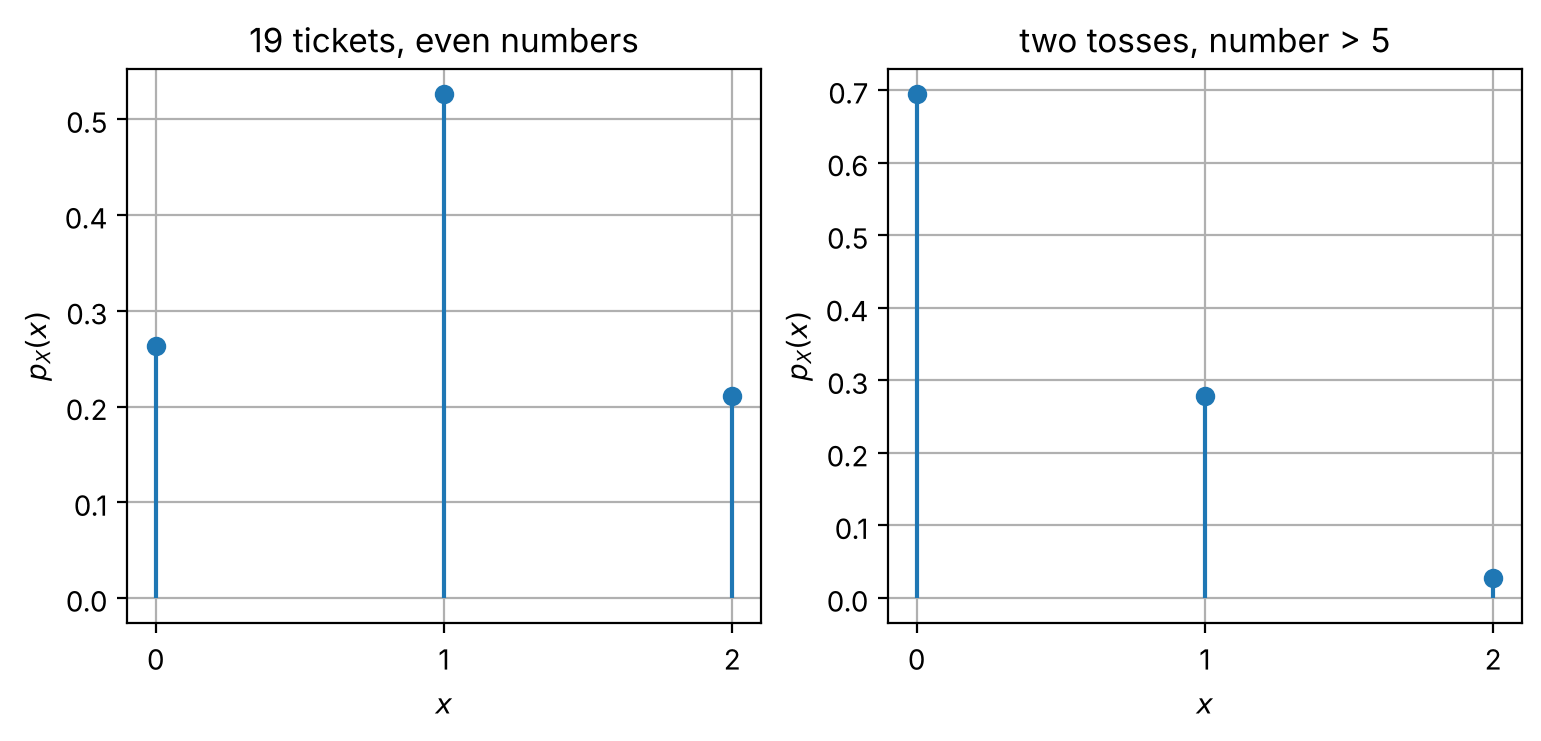
\includegraphics[width=0.80\linewidth]{figs/q23.png}
\caption{pmfs for the tickets (left) and for the die (right)}
\label{fig:cb12-q23}
\end{figure}

\item Solve the following homogeneous differential equation: $x\dfrac{dy}{dx} = x + y$.
\hfill (CBSE XII 65/C/3, Q26)

\solution Put $x = e^t$, so $x\frac{dy}{dx} = \frac{dy}{dt}$ and the equation is $\frac{dy}{dt} - y = e^t$. Taking the Laplace transform from \eqref{eq:cb12-lap1} and \eqref{eq:cb12-laplace},
\begin{align}
sY - y_0 - Y = \frac{1}{s-1} \implies Y(s) = \frac{y_0}{s-1} + \frac{1}{\brak{s-1}^2}
\end{align}
Inverting, $y = \brak{y_0 + t}e^t$, i.e.
\begin{align}
y = x\brak{\log x + C}
\end{align}
The code checks that the numerical transform of $\brak{C+t}e^t$ equals $Y(s)$ (for $C = 0.5$, $s = 3$: $0.5$ on both sides) and solves the equation by the Euler forward method \eqref{eq:cb12-euler}: at $x = 4$ it gives $7.5302$ against $7.5452$. See \figref{fig:cb12-q26}.
\begin{lstlisting}[frame=single, basicstyle=\rmfamily, escapeinside={(*@}{@*)}]
(*@\makebox[\dimexpr\linewidth-2\fboxsep-2\fboxrule\relax][c]{codes/q26.py}@*)
\end{lstlisting}
\begin{figure}[H]
\centering
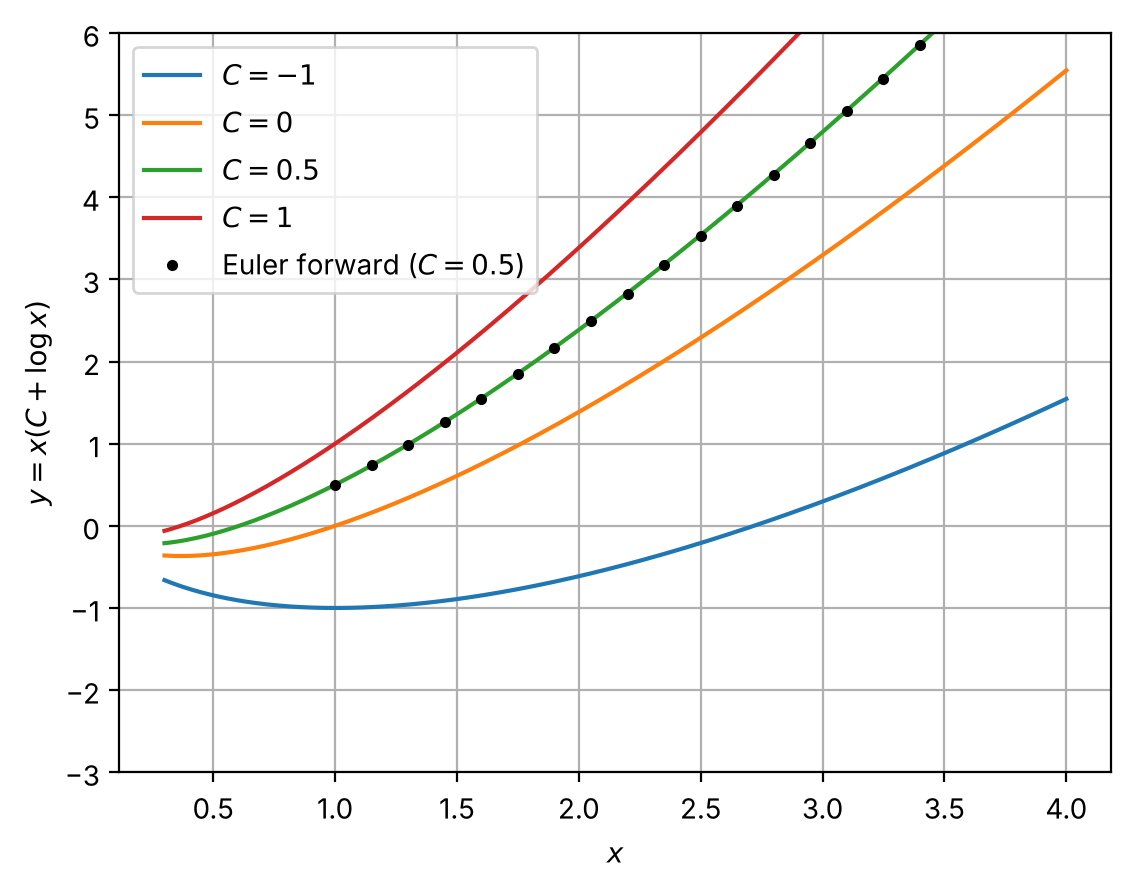
\includegraphics[width=0.65\linewidth]{figs/q26.png}
\caption{Solutions $y = x(C + \log x)$ and the Euler forward method}
\label{fig:cb12-q26}
\end{figure}

\item The random variable $X$ has a probability function $P(x)$ defined below, where $k$ is some number: $P(x) = k$ for $x = 0$, $2k$ for $x = 1$, $3k$ for $x = 2$, and $0$ otherwise. Find (i) the value of $k$, (ii) $P(X < 2)$, $P(X \le 2)$, $P(X \ge 2)$.
\hfill (CBSE XII 65/C/3, Q28)

\solution From \eqref{eq:cb12-pmf} the pmf sums to $1$: $\myvec{1 & 2 & 3}\myvec{k \\ k \\ k} = 6k = 1$, so $k = \frac{1}{6}$ (Gauss elimination on the $1\times 1$ system). The pmf is $\myvec{\frac{1}{6} & \frac{2}{6} & \frac{3}{6}}$ and
\begin{align}
P(X<2) &= \frac{1}{6} + \frac{2}{6} = \frac{1}{2}, \quad P(X \le 2) = 1, \quad P(X \ge 2) = \frac{3}{6} = \frac{1}{2}
\end{align}
The following code verifies this in \figref{fig:cb12-q28}.
\begin{lstlisting}[frame=single, basicstyle=\rmfamily, escapeinside={(*@}{@*)}]
(*@\makebox[\dimexpr\linewidth-2\fboxsep-2\fboxrule\relax][c]{codes/q28.py}@*)
\end{lstlisting}
\begin{figure}[H]
\centering
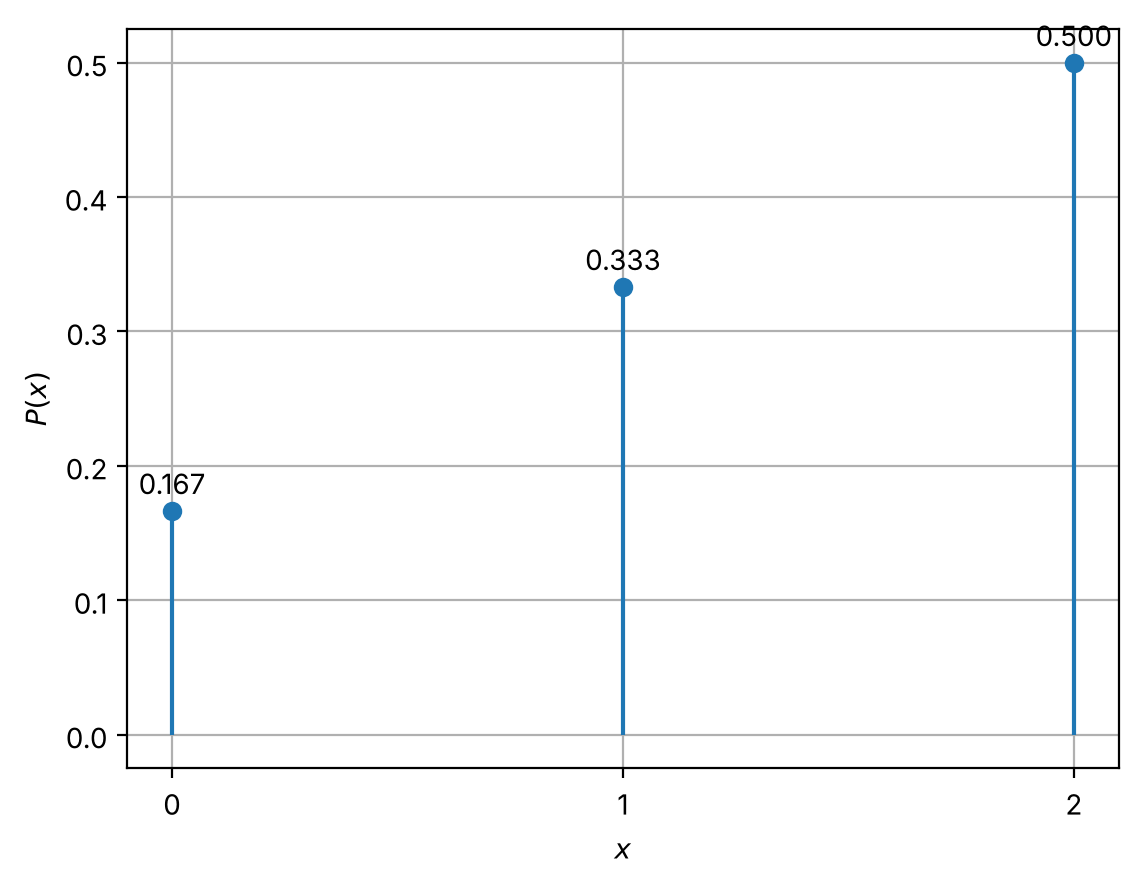
\includegraphics[width=0.50\linewidth]{figs/q28.png}
\caption{pmf of $X$}
\label{fig:cb12-q28}
\end{figure}

\item Find the shortest distance between the following lines and hence write whether the lines are intersecting or not: $\dfrac{x-1}{2} = \dfrac{y+1}{3} = z$, $\dfrac{x+1}{5} = \dfrac{y-2}{1}$, $z = 2$.
\hfill (CBSE XII 65/C/3, Q30)

\hfill OR \\
Find the equation of the plane through the line of intersection of the planes $\vec{r}\cdot\brak{\hat{i} + 3\hat{j}} + 6 = 0$ and $\vec{r}\cdot\brak{3\hat{i} - \hat{j} - 4\hat{k}} = 0$, which is at a unit distance from the origin.

\solution $\vec{p}_1 = \myvec{1 \\ -1 \\ 0}$, $\vec{d}_1 = \myvec{2 \\ 3 \\ 1}$, $\vec{p}_2 = \myvec{-1 \\ 2 \\ 2}$, $\vec{d}_2 = \myvec{5 \\ 1 \\ 0}$, $\vec{w} = \vec{p}_1 - \vec{p}_2 = \myvec{2 \\ -3 \\ -2}$. The normal equations \eqref{eq:cb12-skew} are
\begin{align}
\myvec{14 & -13 \\ 13 & -26}\myvec{s \\ t} = \myvec{-\brak{4 - 9 - 2} \\ -\brak{10 - 3}} = \myvec{7 \\ -7}
\end{align}
Gauss elimination, $R_2 \leftarrow R_2 - \frac{13}{14}R_1$:
\begin{align}
\myvec{14 & -13 & 7 \\ 13 & -26 & -7} \longrightarrow \myvec{14 & -13 & 7 \\ 0 & -\frac{195}{14} & -\frac{189}{14}}
\implies t = \frac{189}{195} = \frac{63}{65}, \quad s = \frac{7 + 13t}{14} = \frac{7}{5}
\end{align}
The closest points are $\vec{p}_1 + s\vec{d}_1 = \myvec{3.8 \\ 3.2 \\ 1.4}$ and $\vec{p}_2 + t\vec{d}_2 = \myvec{3.846 \\ 2.969 \\ 2}$. The shortest distance is
\begin{align}
d = \norm{\brak{\vec{p}_1 + s\vec{d}_1} - \brak{\vec{p}_2 + t\vec{d}_2}} = \frac{9}{\sqrt{195}} \approx 0.6445 \neq 0
\end{align}
so the lines do not intersect.

\textbf{OR:} The planes are $\vec{n}_1 = \myvec{1 \\ 3 \\ 0}$, $c_1 = -6$ and $\vec{n}_2 = \myvec{3 \\ -1 \\ -4}$, $c_2 = 0$. From \eqref{eq:cb12-family}, $\vec{n} = \myvec{1+3\lambda \\ 3-\lambda \\ -4\lambda}$, $c = -6$ and the distance condition $\frac{6}{\norm{\vec{n}}} = 1$ gives
\begin{align}
g\brak{\lambda} = \norm{\vec{n}}^2 - 36 = 26\lambda^2 - 26 = 0
\end{align}
The Newton-Raphson iteration \eqref{eq:cb12-nr}, $\lambda_{n+1} = \lambda_n - \frac{g\brak{\lambda_n}}{52\lambda_n}$, gives $\lambda = \pm 1$ and the planes
\begin{align}
4x + 2y - 4z + 6 = 0, \quad -2x + 4y + 4z + 6 = 0
\end{align}
i.e. $2x + y - 2z + 3 = 0$ and $x - 2y - 2z - 3 = 0$. The following code verifies both parts.
\begin{lstlisting}[frame=single, basicstyle=\rmfamily, escapeinside={(*@}{@*)}]
(*@\makebox[\dimexpr\linewidth-2\fboxsep-2\fboxrule\relax][c]{codes/q30.py}@*)
\end{lstlisting}

\item Find a unit vector perpendicular to each of the vectors $\brak{\vec{a}+\vec{b}}$ and $\brak{\vec{a}-\vec{b}}$ where $\vec{a} = \hat{i} + \hat{j} + \hat{k}$, $\vec{b} = \hat{i} + 2\hat{j} + 3\hat{k}$.
\hfill (CBSE XII 65/C/3, Q31)

\solution $\vec{u} = \vec{a}+\vec{b} = \myvec{2 \\ 3 \\ 4}$, $\vec{v} = \vec{a}-\vec{b} = \myvec{0 \\ -1 \\ -2}$. From \ref{eq:cb12-perp}, with $n_3 = 1$,
the augmented matrix (rows $\vec{u}^{\top}$ and $\vec{v}^{\top}$, right side $-u_3, -v_3$) is already upper triangular:
\begin{align}
\myvec{2 & 3 & -4 \\ 0 & -1 & 2}
\end{align}
Back substitution: $-n_2 = 2 \implies n_2 = -2$, $2n_1 + 3\brak{-2} = -4 \implies n_1 = 1$. So $\vec{n} = \myvec{1 \\ -2 \\ 1}$, $\norm{\vec{n}} = \sqrt{6}$ and the unit vectors are
\begin{align}
\pm\frac{1}{\sqrt{6}}\myvec{1 \\ -2 \\ 1}
\end{align}
The following code verifies $\vec{n}^{\top}\vec{u} = \vec{n}^{\top}\vec{v} = 0$.
\begin{lstlisting}[frame=single, basicstyle=\rmfamily, escapeinside={(*@}{@*)}]
(*@\makebox[\dimexpr\linewidth-2\fboxsep-2\fboxrule\relax][c]{codes/q31.py}@*)
\end{lstlisting}

\item Using properties of determinants show that
\begin{align*}
\mydet{1+a^2-b^2 & 2ab & -2b \\ 2ab & 1-a^2+b^2 & 2a \\ 2b & -2a & 1-a^2-b^2} = \brak{1+a^2+b^2}^3
\end{align*}
\hfill (CBSE XII 65/C/3, Q32)

\hfill OR \\
Find the equation of the line joining $A\brak{1,3}$ and $B\brak{0,0}$ using determinants. Also, find $k$ if $D\brak{k,0}$ is a point such that the area of $\triangle ABD$ is $3$ square units.

\solution Apply $R_1 \leftarrow R_1 + bR_3$ and $R_2 \leftarrow R_2 - aR_3$ (the determinant is unchanged, from \eqref{eq:cb12-det}). With $\Delta = 1 + a^2 + b^2$,
\begin{align}
\mydet{\Delta & 0 & -b\Delta \\ 0 & \Delta & a\Delta \\ 2b & -2a & 1-a^2-b^2} &= \Delta^2\mydet{1 & 0 & -b \\ 0 & 1 & a \\ 2b & -2a & 1-a^2-b^2}
\end{align}
Expanding the last determinant along the first row,
\begin{align}
\brak{1 - a^2 - b^2 + 2a^2} + \brak{-b}\brak{0 - 2b} = 1 + a^2 + b^2 = \Delta
\end{align}
so the value is $\Delta^3 = \brak{1+a^2+b^2}^3$. $\blacksquare$ The code checks it by cofactor expansion for random $a, b$.

\textbf{OR:} $\vec{n} = \myvec{0 & 1 \\ -1 & 0}\brak{\vec{A}-\vec{B}} = \myvec{3 \\ -1}$ and the line is $\vec{n}^{\top}\vec{x} = 0$, i.e. $3x - y = 0$. From \eqref{eq:cb12-area}, the area is $\frac{1}{2}\abs{\vec{n}^{\top}\myvec{k \\ 0}} = \frac{3\abs{k}}{2} = 3$, so $k = \pm 2$. The following code verifies this.
\begin{lstlisting}[frame=single, basicstyle=\rmfamily, escapeinside={(*@}{@*)}]
(*@\makebox[\dimexpr\linewidth-2\fboxsep-2\fboxrule\relax][c]{codes/q32.py}@*)
\end{lstlisting}

\item Evaluate $\displaystyle\int_1^3\brak{x^2 + 1 + e^x}dx$ as the limit of sums.
\hfill (CBSE XII 65/C/3, Q34)

\solution With $h = \frac{2}{n}$ and $f(x) = x^2 + 1 + e^x$,
\begin{align}
\int_1^3 f\,dx &= \lim_{n\to\infty}h\sum_{i=1}^{n}f\brak{1+ih} \\
&= \lim_{n\to\infty}h\sbrak{2n + 2h\frac{n\brak{n+1}}{2} + h^2\frac{n\brak{n+1}\brak{2n+1}}{6} + e\frac{e^h\brak{e^{nh}-1}}{e^h - 1}}
\end{align}
Using $nh = 2$ and $\frac{h}{e^h-1} \to 1$, the limit is $4 + 4 + \frac{8}{3} + e\brak{e^2 - 1}$, so
\begin{align}
\int_1^3 f\,dx &= \frac{32}{3} + e^3 - e \approx 28.03392
\end{align}
The trapezoidal rule \eqref{eq:cb12-trap} gives $28.4776$ for $N = 4$, $28.0357$ for $N = 64$ and $28.03392$ for $N = 16384$, converging to the same value. The following code verifies this.
\begin{lstlisting}[frame=single, basicstyle=\rmfamily, escapeinside={(*@}{@*)}]
(*@\makebox[\dimexpr\linewidth-2\fboxsep-2\fboxrule\relax][c]{codes/q34.py}@*)
\end{lstlisting}

\item If $y = x^{\sin x} + \sin^{-1}\sqrt{x}$, then find $\dfrac{dy}{dx}$.
\hfill (CBSE XII 65/C/3, Q36)

\solution Let $y_1 = x^{\sin x}$, so $\log y_1 = \sin x\log x$ and $\frac{y_1'}{y_1} = \cos x\log x + \frac{\sin x}{x}$. Also $\frac{d}{dx}\sin^{-1}\sqrt{x} = \frac{1}{\sqrt{1-x}}\cdot\frac{1}{2\sqrt{x}}$. Hence
\begin{align}
\frac{dy}{dx} = x^{\sin x}\brak{\cos x\log x + \frac{\sin x}{x}} + \frac{1}{2\sqrt{x\brak{1-x}}}
\end{align}
\textbf{Laplace transform:} on $x = 0.25 + t$, $t \in \sbrak{0, 0.5}$, the property \eqref{eq:cb12-lap1} on a finite interval reads $L\{y'\} = sY(s) - y(0) + e^{-sT}y(T)$. The code evaluates $Y(s)$ with the trapezoidal rule: at $s = 2$ both sides equal $0.381810$; at $s = 5$ both equal $0.206807$. The Euler forward difference \eqref{eq:cb12-euler-diff} gives $0.975397, 1.251443, 1.605675$ at $x = 0.3, 0.5, 0.7$ against the formula values $0.975396, 1.251442, 1.605674$.
\begin{lstlisting}[frame=single, basicstyle=\rmfamily, escapeinside={(*@}{@*)}]
(*@\makebox[\dimexpr\linewidth-2\fboxsep-2\fboxrule\relax][c]{codes/q36.py}@*)
\end{lstlisting}

\end{enumerate}


\end{document}
